%==============================================================================
% IEEE journal manuscript — project skeleton (placeholder content).
% Document class: IEEEtran (official). Body is migrated in a later phase.
%
% Build:  pdflatex main  ->  bibtex main  ->  pdflatex main  ->  pdflatex main
% (see README.md for a one-line latexmk command and for IEEEtran.cls provenance)
%==============================================================================
\documentclass[journal]{IEEEtran}

% ---- Packages -------------------- ------------------------------------------
\usepackage[T1]{fontenc}             % proper glyphs for accented names
\usepackage[utf8]{inputenc}          % input encoding (portable on older TeX)
\usepackage{cite}                    % IEEE-style reference handling
\usepackage{amsmath}                 % equations
\usepackage{amssymb}                 % math symbols
\usepackage{graphicx}                % figures
\graphicspath{{figures/}}            % figure search path
\usepackage{booktabs}                % professional tables (\toprule etc.)
\usepackage{multirow}                % multi-row table cells
\usepackage{subcaption}              % multi-panel figures (Figs. 3, 5, 6)
\usepackage{url}
\usepackage[hidelinks]{hyperref}     % load last; internal/external links
% Improve display equation spacing for IEEE two-column layout
\setlength{\abovedisplayskip}{8pt plus 2pt minus 2pt}
\setlength{\belowdisplayskip}{8pt plus 2pt minus 2pt}
\setlength{\abovedisplayshortskip}{6pt plus 2pt minus 2pt}
\setlength{\belowdisplayshortskip}{6pt plus 2pt minus 2pt}

% ---- Front matter ----------------------------------------------------------
\begin{document}

\title{A Dual-Stream Spatial--Spectral Fusion Pathway for\\
       Boundary Fidelity in Dermoscopic Skin Lesion Segmentation}

\author{
\begin{tabular}{c c}
Samartha H V &  Shreyas J \\
\textit{Manipal Institute of Technology Bengaluru,} &
\textit{Manipal Institute of Technology Bengaluru,} \\
\textit{Manipal Academy of Higher Education,} &
\textit{Manipal Academy of Higher Education,} \\
Manipal, India & Manipal, India \\
samartha1.mitblr2025@learner.manipal.edu &
shreyas.j@manipal.edu \\
\end{tabular}
}

%\markboth{IEEE Transactions on Placeholder,~Vol.~XX, No.~XX, Month~2026}%
{Author \MakeLowercase{\textit{et al.}}: Dual-Stream Spatial--Spectral Fusion for Dermoscopic Segmentation}

\maketitle

% ---- Abstract & keywords ---------------------------------------------------
\begin{abstract}
Accurate delineation of lesion boundaries remains a fundamental difficulty in dermoscopic image segmentation, where gradual lesion-to-skin transitions, irregular margins, and occluding structures such as hair make the contour the least certain part of any prediction. Segmentation methods are nevertheless optimised and assessed predominantly by region-overlap criteria, which are area-based and respond only weakly to displacement of the contour; boundary-relevant content is commonly merged with contextual information in a single representation dominated by the lesion interior. This paper presents a targeted refinement of the MAFF-Net framework in which the pretrained encoder, decoder, and auxiliary reconstruction branch are retained and only the fusion pathway is redesigned. Multi-scale features from a frozen foundation backbone are processed along two parallel streams, a spatial stream that preserves contextual structure and a parameter-free frequency stream that emphasises boundary-sensitive spectral content; their statistics are reconciled before they are merged by a learned, spatially varying gate. The method was evaluated on three public dermoscopic benchmarks against four segmentation architectures under an identical protocol, using region-based and boundary-based measures in combination, and each introduced component was isolated by a leave-one-out ablation. Removing any component degraded all boundary measures while leaving region overlap substantially unchanged. The contribution is accordingly characterised as an improvement in boundary fidelity rather than region overlap, and indicates that region-overlap criteria alone are insufficient to assess methods acting upon the lesion margin. All results derive from single training runs, and no claim of statistical significance is made.
\end{abstract}


\begin{IEEEkeywords}
Skin lesion segmentation, dermoscopy, boundary fidelity, frequency-domain
representation, gated feature fusion, frozen foundation model, deep supervision,
ISIC.
\end{IEEEkeywords}

\IEEEpeerreviewmaketitle

% ---- Body (one file per section) -------------------------------------------
\section{Introduction}
\label{sec:intro}

Skin cancer is among the most frequently diagnosed malignancies worldwide, and melanoma, though less common than the keratinocyte carcinomas, accounts for a disproportionate share of the associated mortality \cite{ref1}. Because prognosis depends strongly on the stage at detection --- lesions caught while still confined to the epidermis carry markedly more favourable outcomes than those found after invasion --- early and accurate identification of suspicious pigmented lesions is of considerable clinical importance. The diagnostic burden nonetheless falls on a specialist workforce that is small relative to the volume of lesions requiring assessment, which has drawn sustained attention to computational methods that support their examination.

Dermoscopy, a non-invasive technique that suppresses surface reflection to reveal subsurface pigmented structures, is now a routine modality in this assessment \cite{ref2}, and segmentation of the lesion region is a foundational step within it. The delineated region fixes the measured extent and shape of the lesion, which underpin the morphological criteria --- asymmetry, border irregularity, and diameter --- of established diagnostic rules \cite{ref3}, and it further conditions downstream classification systems that operate on the region or on features derived from it. Manual delineation, however, is laborious and varies appreciably between observers, most of all along the lesion margin, which motivates automated methods.

That margin is the crux of the task. Dermoscopic images frequently show low contrast between lesion and skin, so the transition is gradual rather than abrupt and cannot be located from local intensity gradients alone; margins are often diffuse or irregular, fading into adjacent skin over an extended transition zone. Structures that are not part of the lesion --- hair, air bubbles, ruler markings, and vascular patterns --- may traverse or obscure the boundary \cite{ref2}, and a single image may contain more than one pigmented structure, while lesions vary widely in scale, shape, colour, and texture. These conditions bear most heavily on the boundary, where the evidence separating lesion from background is weakest.

Automated approaches have developed along two lines. Convolutional encoder--decoder networks, archetypally the U-Net \cite{ref4}, join contracting and expanding paths by skip connections, and were later refined through attention gating of those connections \cite{ref5}, nested and densely connected decoders \cite{ref6}, and multi-scale aggregation; these capture local structure well, but the limited receptive field of convolution restricts their access to long-range context. Self-attention architectures answered this limitation, either replacing the convolutional encoder with a vision transformer \cite{ref7} or combining convolutional and transformer components in hybrid encoders \cite{ref8}, admitting global context at appreciably greater computational and data cost. More recently, large-scale visual foundation models --- most prominently the Segment Anything Model family \cite{ref9,ref10} --- have been adapted to medical segmentation, their image encoders supplying transferable representations that reduce the dependence on scarce annotated data.

Each line leaves difficulties that bear directly on boundary delineation. Foundation models, trained predominantly on natural images, are separated from dermoscopy by a domain gap \cite{ref11}, so that the adaptation mechanism rather than the backbone governs how faithfully fine structure is preserved. More fundamentally, most methods are both optimised and evaluated by region-overlap criteria. These are area-based, and the contour neighbourhood occupies only a small fraction of a compact lesion, so a contour displaced by a small distance alters the overlapping area only slightly \cite{ref12}; optimisation and evaluation on this basis exert little pressure on the very region where dermoscopic segmentation is hardest, and can fail to separate methods whose contours differ appreciably. Where boundary-sensitive content is treated at all, it is usually handled implicitly, merged with contextual information in a single undifferentiated representation dominated by the low-frequency interior.

Two remedies follow directly. Boundary-relevant content can be represented explicitly in the frequency domain, where the intensity transitions of lesion margins occupy the higher-frequency band \cite{ref13,ref14} and separate from the low-frequency interior more cleanly than in a single spatial representation; and it can be assessed explicitly with measures defined on the contour, since region overlap alone cannot characterise it. The Original MAFF-Net \cite{ref15} moved in this direction, adapting a frozen foundation backbone to dermoscopy through multi-scale perception adaptation and frequency-guided feature fusion with an auxiliary reconstruction branch, and demonstrating that spatial and spectral information can be integrated effectively. It does not, however, maintain the spatial and frequency representations as separate streams that are statistically reconciled before they are combined; closing that gap --- fusing the two domains as explicitly separated, reconciled streams --- motivates the present work.

Accordingly, this work investigates a targeted dual-stream refinement of the fusion stage of the MAFF-Net framework, rather than a replacement of the framework as a whole. The pretrained encoder, the convolutional decoder, and the auxiliary reconstruction branch are retained from the Original MAFF-Net, and the redesign is confined to the pathway in which spatial and spectral information are combined. The multi-scale features produced by the frozen encoder are routed simultaneously along a spatial stream, which preserves regional and contextual structure, and a frequency stream, which emphasises boundary-sensitive spectral content; the two are brought onto a common statistical footing and then merged by a learned gate whose weighting is inferred from the features themselves rather than fixed in advance. Training combines a region objective with auxiliary boundary-focused supervision applied to the segmentation outputs and to the reconstruction branch. The resulting model is evaluated against standard convolutional and transformer baselines under a protocol that reports region-based and boundary-based measures together, so that its effect on the lesion contour is assessed separately from its effect on the extent of the predicted region.

The contributions are threefold. First, region-overlap metrics alone are shown to be insufficient to characterise methods that act on the lesion margin: evaluating the models on the held-out test splits of three public dermoscopic benchmarks with region-based and boundary-based measures in combination yields different rankings under the two families of measures, so that boundary quality must be assessed with contour-based measures rather than inferred from region overlap. Second, the proposed dual-stream model --- a parameter-free Frequency Branch, per-stream Feature Alignment, and a learned Gated Fusion on a frozen foundation backbone --- attains higher region-based and boundary-based scores than four standard convolutional and transformer baselines on all three benchmarks under an identical single-run protocol. Third, the dual-stream reformulation of the fusion pathway is investigated, and a leave-one-out ablation isolates the marginal role of its three components: disabling any one degrades all boundary measures while leaving region overlap essentially unchanged on the dataset examined, confining their effect to boundary fidelity rather than to the extent of the predicted region. The encoder, decoder, and reconstruction branch are adopted from the Original MAFF-Net and are not claimed as contributions of this work; the boundary-centric supervision under which the network is trained is described in Section III-H as part of the training objective.

The remainder of the paper is organised as follows. Section II reviews related work on dermoscopic lesion segmentation; Section III presents the proposed methodology; Section IV specifies the datasets, implementation, evaluation measures, and experimental protocol; Section V reports the results; Section VI discusses their interpretation and the limitations of the study; and Section VII concludes.

\section{Related Work}
\label{sec:related}

\subsection{Convolutional Segmentation Architectures}

The formulation of segmentation as dense per-pixel classification by fully convolutional networks \cite{ref16} established the basis upon which subsequent architectures were constructed. The U-Net \cite{ref4} adapted this formulation to biomedical imaging by pairing a contracting encoder with a symmetric expanding decoder and joining the two by skip connections, so that the fine spatial detail lost to successive downsampling could be reintroduced during reconstruction. This design proved well suited to the small annotated datasets characteristic of medical imaging and remains the reference point for the field. Later work observed that the direct concatenation of encoder and decoder features couples representations of differing semantic level, and UNet++ \cite{ref6} accordingly interposed a nested arrangement of dense convolutional blocks along the skip pathways in order to reduce this disparity. These architectures recover the lesion region reliably, but the locality of the convolution operator restricts the spatial extent over which evidence can be aggregated, which is a limitation where the margin must be inferred from context beyond its immediate neighbourhood.

\subsection{Attention Mechanisms}

Attention mechanisms were introduced into this setting as a means of weighting features according to their informativeness rather than treating them uniformly. Squeeze-and-excitation blocks \cite{ref17} recalibrate feature channels by a globally pooled descriptor, allowing informative channels to be emphasised. The Attention U-Net \cite{ref5} applies a related principle spatially, gating each skip connection so that regions irrelevant to the target are suppressed before the encoder features are passed to the decoder. Such mechanisms improve the selectivity of the representation, and the gating principle they establish --- that the contribution of a feature should be determined from the feature itself rather than fixed in advance --- is directly relevant to the combination of heterogeneous representations. They do not, however, alter the receptive field of the underlying convolutions, and the constraint on long-range aggregation persists.

\subsection{Transformer-Based Segmentation}

The vision transformer \cite{ref7} addressed this constraint by dispensing with convolution in favour of self-attention over image patches, admitting global interactions at every layer. Because pure transformer encoders forgo the inductive biases that make convolutional networks efficient on limited data, hybrid designs were proposed for medical segmentation. TransUNet \cite{ref8} employs a convolutional encoder followed by transformer layers and retains a convolutional decoder, thereby combining local feature extraction with global context modelling, while Swin-UNet \cite{ref18} constructs an encoder--decoder entirely from hierarchical windowed attention blocks. These architectures capture context effectively, but they carry substantially greater computational and data requirements, which is a material consideration given the size of publicly available dermoscopic collections.

\subsection{Foundation Models for Medical Segmentation}

The difficulty of training large models on limited annotated data has motivated the adaptation of visual foundation models pretrained on very large and diverse collections. The Segment Anything Model \cite{ref9} provides a promptable architecture whose image encoder yields broadly transferable representations, and its successor \cite{ref10} extends the family with a hierarchical encoder and improved efficiency. Direct application to medical images is nevertheless impaired by the domain gap between natural and medical imagery, and adaptation is required; MedSAM \cite{ref11} addresses this by fine-tuning on a large assembled corpus of medical images. Fine-tuning an encoder of this scale is costly and, on small datasets, carries a risk of overfitting, which has led to approaches that retain the encoder in a frozen state and confine the trainable capacity to modules operating on its outputs. Under such a scheme the adaptation mechanism, rather than the backbone, governs how faithfully fine structure is preserved.

\subsection{Frequency-Domain Learning}

A complementary line of work processes features in the frequency domain rather than the spatial domain alone. Fast Fourier convolution \cite{ref13} incorporates a spectral branch within the convolutional block so that a global receptive field is obtained at modest cost, and global filter networks \cite{ref14} replace self-attention outright with learnable filters applied to the Fourier transform of the feature map. The interest of these methods for boundary delineation lies in the correspondence between spectral content and spatial structure: abrupt intensity transitions of the kind associated with object margins are represented predominantly in the higher-frequency components, whereas the smoothly varying appearance of homogeneous regions is concentrated in the lower-frequency components. Operating in this domain therefore affords a means of addressing margin-related content more directly than is possible within a single spatial representation.

\subsection{Boundary-Aware Segmentation}

Recognition that region-overlap objectives exert limited pressure upon the contour has prompted the development of boundary-aware formulations. Boundary loss \cite{ref19} supplements a region objective with a distance-weighted term computed from the ground-truth contour, and related work has sought to reduce contour distances directly during optimisation. A parallel concern arises in evaluation: region-overlap criteria are area-based and are correspondingly insensitive to modest displacements of the contour, so that methods differing appreciably in margin fidelity may be assigned similar scores. The Boundary IoU measure \cite{ref12} was proposed in response, restricting the overlap computation to a band about the contour so that boundary quality is assessed separately from region extent. Distance-based measures such as the Hausdorff distance and the average symmetric surface distance serve a comparable purpose in medical image analysis.

\subsection{Summary and Research Gap}

These lines of work converge upon the framework from which the present study proceeds. The Original MAFF-Net \cite{ref15} adapts a frozen foundation backbone to dermoscopic segmentation through multi-scale perception adaptation and frequency-guided feature fusion, together with an auxiliary reconstruction branch, and demonstrates that spatial and spectral information can be integrated productively within a single framework. Three observations nevertheless remain. First, in that design and in comparable approaches the spectral and spatial content are combined within one fusion route rather than being maintained as separate streams; representations of markedly different statistical character are thereby merged without prior reconciliation, and the low-frequency content describing the lesion interior may predominate. Second, where two heterogeneous representations are combined, the weighting between them is commonly fixed rather than determined from the features themselves, notwithstanding that the gating principle established in the attention literature is directly applicable. Third, and cutting across the foregoing, methods intended to improve margin delineation are still assessed principally by region-overlap criteria, which, for the reasons set out above, are ill-suited to detecting the very property such methods are designed to improve.

The present work addresses these three points together. It retains the frozen foundation backbone and the established decoding pathway, separates the spatial and spectral representations into parallel streams, reconciles their statistics before combination, and merges them by a learned gate whose weighting varies with the features presented to it. It further evaluates the resulting model with region-based and boundary-based measures in combination, so that the effect upon the contour may be observed independently of the effect upon region extent.

\section{Methodology}
\label{sec:method}

\subsection{Overall Framework of the Proposed MAFF-Net}

Accurate delineation of the lesion region in dermoscopy is a prerequisite for downstream tasks such as morphological assessment, malignancy scoring, and treatment planning, yet manual delineation is time-consuming and varies between observers, which motivates reliable automated segmentation. The task remains difficult because dermoscopic images frequently exhibit low contrast between lesion and surrounding skin, gradual or ill-defined boundaries, occlusion by hair and vascular structures, and pronounced variability in lesion shape, scale, and pigmentation. Methods intended for clinical support must therefore remain robust under these conditions and, in particular, must recover lesion boundaries faithfully.

Large-scale visual foundation models supply transferable representations that reduce the dependence on scarce annotated medical data, but their direct application to dermoscopy is limited by the domain gap between natural and medical images. The Original MAFF-Net \cite{ref15} addresses this gap by adapting a pretrained foundation backbone with multi-scale perception adaptation (MMPA) and frequency-guided feature fusion (FGFF), and by regularising the decoder through an auxiliary Reconstruction Decoder Branch (RDB). This design integrates spatial and spectral information effectively but does not explicitly separate the spatial and frequency representations prior to fusion, which motivates an explicit dual-stream integration in which the two domains are treated as separate, reconciled streams.

Accordingly, this work pursues a targeted refinement of the MAFF-Net framework rather than its replacement: the validated components of the Original MAFF-Net are retained and only the fusion pathway is redesigned, where explicit dual-stream integration is justified. The frozen encoder, the convolutional decoder, and the auxiliary reconstruction branch are preserved without alteration, so that the transferable priors and the proven decoding pathway continue to anchor the network. In place of the original single fusion pathway, the multi-scale features produced by the encoder are processed along two parallel routes: a spatial stream that preserves regional and contextual structure, and a frequency stream that emphasises boundary-sensitive detail. Fig.~\ref{fig:architecture} presents the overall organisation of the Proposed MAFF-Net, in which the two streams are reconciled and combined into a unified representation before decoding.

\begin{figure*}[!t]
\centering
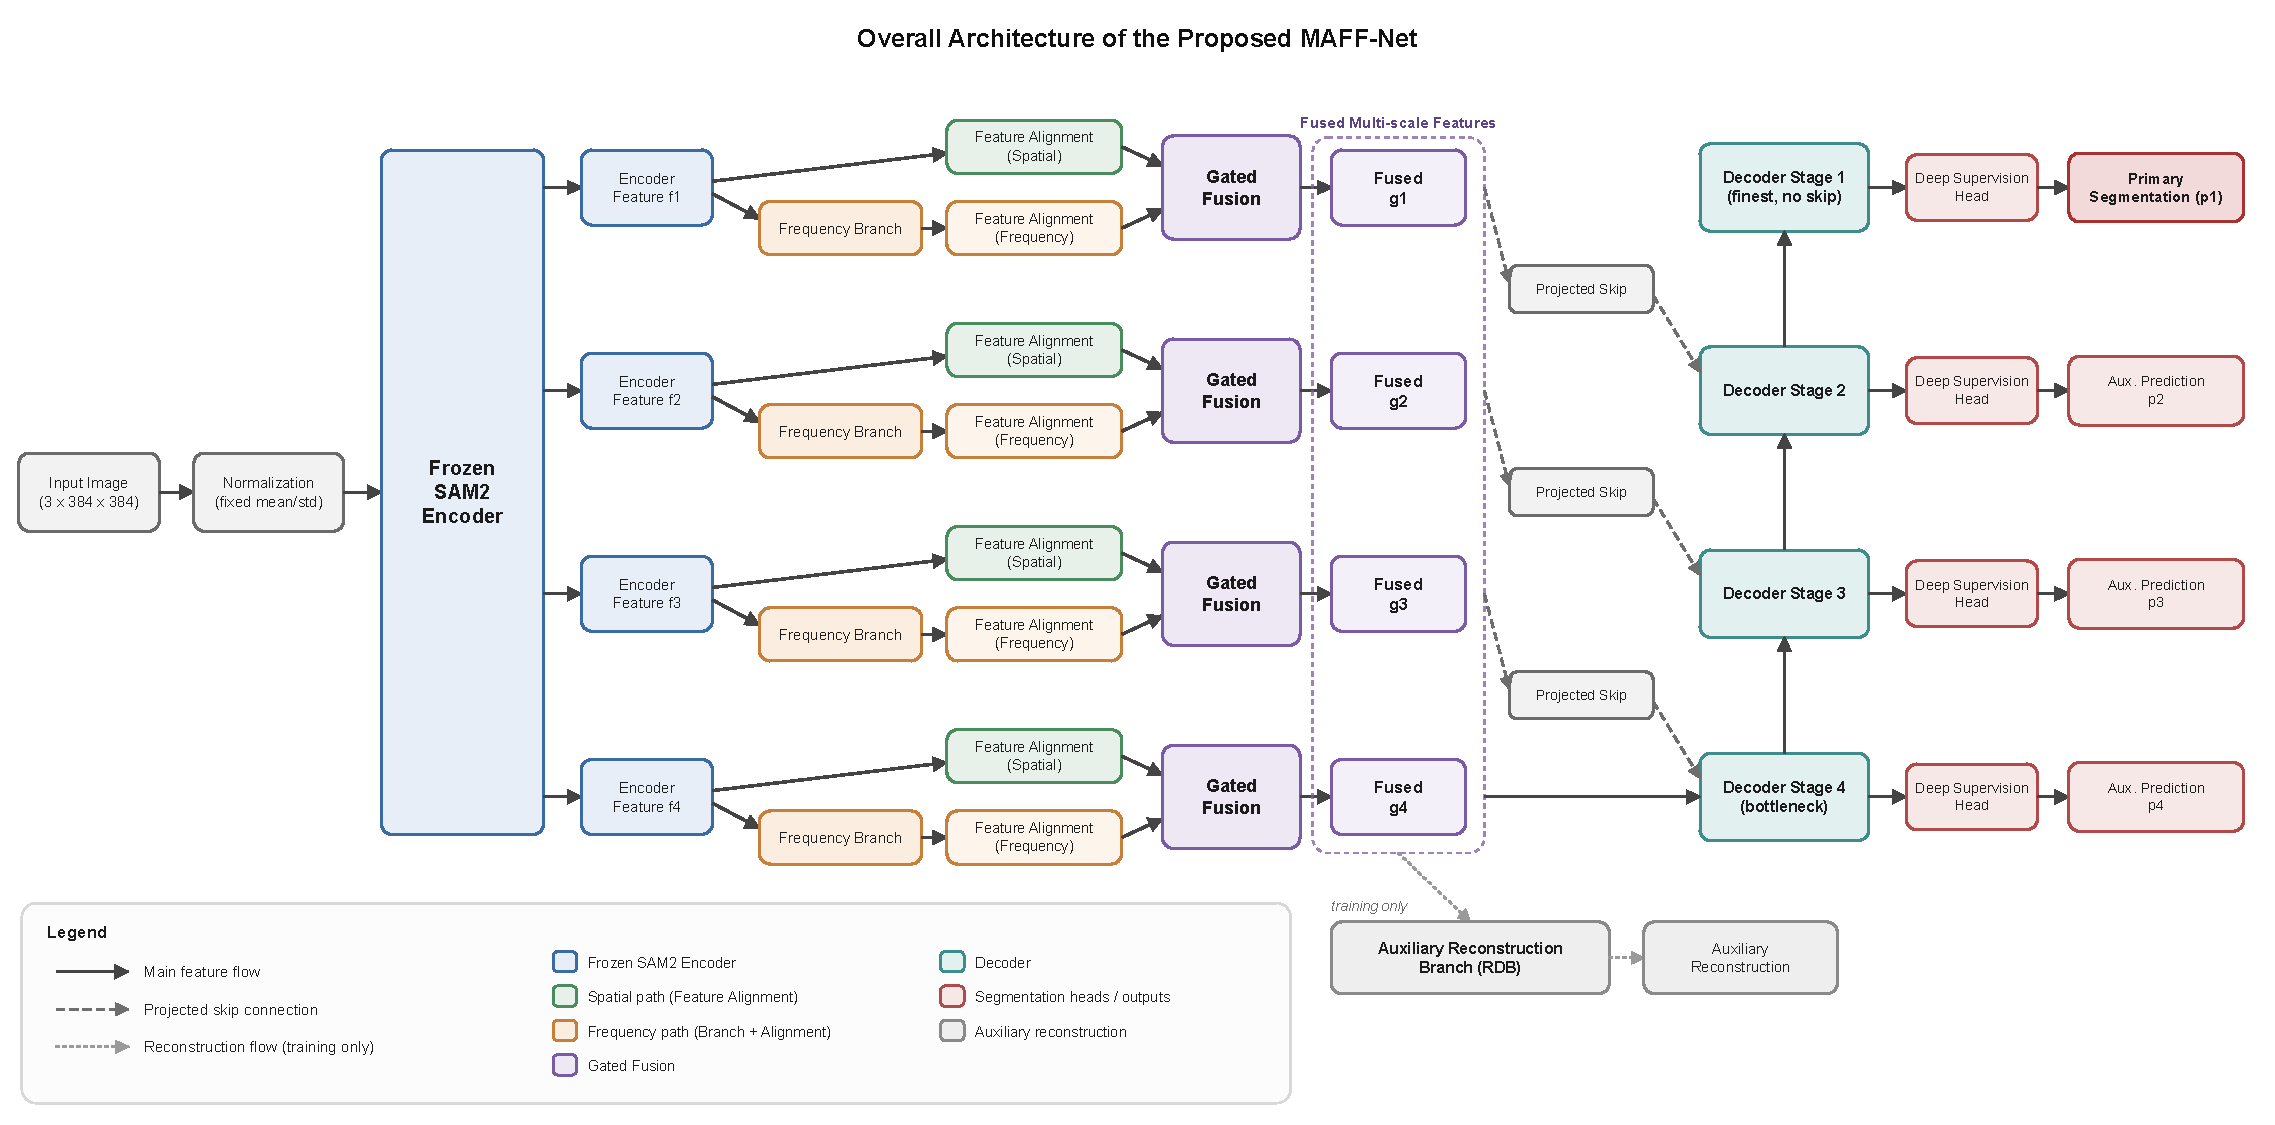
\includegraphics[width=\textwidth]{Figure1_Architecture.pdf}
\caption{Overall architecture of the Proposed MAFF-Net. A frozen SAM2 encoder
produces four multi-scale features, each processed by parallel spatial and
frequency pathways whose aligned representations are combined by gated fusion.
The three shallower fused features enter the decoder through projected skip
connections and the deepest enters as the decoder bottleneck; four
deep-supervision heads produce the segmentation outputs, of which the
highest-resolution one is the primary prediction, and an auxiliary
reconstruction branch operates on the fused features during training.}
\label{fig:architecture}
\end{figure*}

The processing pipeline proceeds as follows. A dermoscopic image is passed through the frozen encoder, yielding a set of multi-scale feature representations; at each scale, the corresponding feature is routed simultaneously into the spatial and frequency streams, so that contextual and boundary-oriented information are extracted in parallel rather than entangled. The two streams are reconciled and combined into a unified representation at each scale, and these fused multi-scale representations are propagated to the convolutional decoder, which produces the lesion segmentation map. During training, the auxiliary reconstruction branch operates alongside the decoder to regularise the learned features and supervision is applied at multiple decoder stages; at inference, only the primary segmentation output is retained.

The components introduced in the fusion pathway are stated here without implementation detail. The Frequency Branch provides an explicit spectral route that emphasises boundary-related content within each encoder feature; the Feature Alignment Module harmonises the statistics of the spatial and frequency representations so that they can be combined consistently; and the Gated Fusion Module replaces implicit fusion with a learned, lightweight combination of the two aligned streams. The network is additionally trained under Boundary-aware Deep Supervision (BDS) and Edge-weighted Reconstruction (EWR), jointly referred to as Boundary-centric Dual Supervision (BcDS), which direct the optimisation toward the lesion contour. The encoder, decoder, and reconstruction branch are preserved from the Original MAFF-Net and are not claimed as contributions of this work.

Taken together, these components constitute a framework that separates spatial and spectral processing, reconciles the two domains before fusion, and reinforces boundary fidelity through BcDS while continuing to rely on the pretrained backbone. The remaining subsections describe each element in detail, beginning with the frozen encoder that produces the multi-scale features on which the two streams operate.

\subsection{Overall Network Architecture}

The Proposed MAFF-Net is a dual-stream encoder--decoder network built on a pretrained visual foundation backbone. Its guiding architectural principle is a clear separation of responsibilities: the encoder supplies transferable multi-scale representations, two parallel pathways process complementary aspects of them, a dedicated stage reconciles and combines the two pathways, and a convolutional decoder produces the segmentation output. The frozen encoder, the convolutional decoder, and the auxiliary reconstruction mechanism are preserved from the Original MAFF-Net, and the redesign is confined to the pathway responsible for combining spatial and spectral information. The network is therefore best understood as a structured composition of preserved and newly introduced components, each assigned a distinct role in the overall processing chain, rather than a monolithic model.

The complete architecture is illustrated in Fig.~\ref{fig:architecture}, which depicts the end-to-end structure of the Proposed MAFF-Net from the input dermoscopic image to the predicted segmentation map. As shown, an input image is first encoded into a set of multi-scale feature representations by the frozen encoder. Each representation is then dispatched to two parallel pathways --- a spatial pathway that retains regional and contextual structure and a frequency pathway that emphasises boundary-sensitive content --- which are reconciled by the Feature Alignment Module and merged by the Gated Fusion Module into a single fused representation at each scale. The fused representations pass to the convolutional decoder, which aggregates information across scales to yield the segmentation map, while an auxiliary reconstruction branch operates alongside the decoder as a training-time regularisation signal; it runs on every forward pass, and at inference its output is discarded and only the primary segmentation output is retained.

At the level of module organisation, the network comprises three functional groups. The first is the preserved backbone: the frozen encoder, adopted from the Original MAFF-Net, which supplies hierarchical multi-scale features and is not adapted during training. The second is the newly introduced fusion pathway, which replaces the single fusion route of the Original MAFF-Net and comprises the Frequency Branch, the Feature Alignment Module, and the Gated Fusion Module. The third comprises the preserved decoding and regularisation components: the convolutional decoder that reconstructs spatial resolution and produces the prediction, and the auxiliary reconstruction branch that constrains the learned features during training. Supervision of the network is governed by Boundary-centric Dual Supervision, which comprises Boundary-aware Deep Supervision and Edge-weighted Reconstruction.

The resulting information flow is a parallel-then-merge structure: at every scale the encoder features fan out into the two pathways so that contextual and boundary-oriented information are extracted concurrently rather than in a single entangled route, are reconciled onto a shared footing by the Feature Alignment Module, and are collapsed back into a single fused stream by the Gated Fusion Module before decoding. The convolutional decoder integrates the fused multi-scale representations from coarse to fine to recover the full-resolution map; during training, the auxiliary reconstruction branch draws on the same fused features to encourage stable and informative representations, while deep supervision at multiple decoder stages guides the intermediate predictions toward the target. In sum, the representation is split into complementary pathways, reconciled, fused, and finally decoded.

The rationale follows from the difficulties of dermoscopic segmentation. Separating the spatial and frequency pathways provides explicit access to boundary-related spectral content while retaining the contextual structure needed to localise the lesion, addressing the low contrast and ill-defined boundaries characteristic of these images. Aligning the pathways before fusion is intended to ensure that representations of different origin are combined on compatible terms, and delegating the combination to a learned gate allows the network to weigh the two domains adaptively rather than committing to a fixed rule. Retaining the pretrained backbone preserves the transferable priors that mitigate the scarcity of annotated dermoscopic data, and retaining the established decoder and reconstruction branch keeps a proven decoding pathway intact, so that the observed behaviour of the network can be attributed to the redesigned fusion pathway and the boundary-centric supervision rather than to changes in the backbone or decoder. This maintains continuity with the philosophy of the Original MAFF-Net, in which a strong frozen encoder is adapted for the medical domain rather than trained from scratch.

Having established the blueprint, the module organisation, and the information flow, the following subsections describe each component in detail --- the frozen encoder, the Frequency Branch, the Feature Alignment Module, the Gated Fusion Module, and the decoder with its auxiliary reconstruction branch --- concluding with the training objective that implements Boundary-centric Dual Supervision.

\subsection{Frozen Foundation Backbone}

Visual foundation models pretrained on large and diverse image collections provide transferable representations that are difficult to obtain from the limited annotated data available in dermoscopy. The Segment Anything Model (SAM) family \cite{ref9}, in particular, is trained at a scale that yields general-purpose spatial priors, and the Original MAFF-Net showed that such a model can be adapted to skin-lesion segmentation by retaining its image encoder as a fixed feature extractor rather than training a network from scratch. Preserving a pretrained backbone in this manner offers two practical advantages that are especially relevant in the medical setting: it transfers robust representations learned from abundant natural images, and it avoids the risk of overfitting and the substantial cost of updating a very large encoder on a comparatively small medical dataset. The Proposed MAFF-Net preserves this design choice without alteration; the SAM2 image encoder \cite{ref10} is adopted from the Original MAFF-Net and used as the feature-extraction foundation of the network.

Within the architecture, the backbone maps the input dermoscopic image, standardised to the statistics expected by the encoder, into a set of intermediate feature representations. Its parameters are frozen throughout training --- neither updated by the optimisation process nor otherwise modified in this work --- so the trainable capacity of the network is concentrated entirely in the modules that operate downstream of it, and the representations it produces remain stable and consistent across training. The encoder is thus used exactly as provided, and none of the contributions claimed in this paper reside within it.

A property important for lesion segmentation is that the backbone is hierarchical, producing representations at several spatial resolutions and semantic levels rather than a single feature map: the shallower representations retain fine spatial detail and are informative about local structure, whereas the deeper ones encode coarser, more semantic context describing the lesion as a whole. This range of scales is well suited to dermoscopic images, in which lesions vary considerably in size and in which accurate delineation requires both localisation of the overall lesion region and sensitivity to fine boundary structure. By spanning these scales, the frozen encoder supplies the multi-scale information on which the subsequent scale-adaptive processing depends, and it does so uniformly for every input without any scale-specific tuning.

These multi-scale representations are the common input to all downstream components of the Proposed MAFF-Net, and it is at this point that the contributions of the present work begin. Each representation is routed into the two parallel pathways, aligned, and combined before decoding, so that the spatial pathway, the Frequency Branch, the Feature Alignment Module, and the Gated Fusion Module all operate on the encoder outputs rather than on the raw image. Redesigning or fine-tuning the backbone is unnecessary for the goals of this study, because the limitation motivating the proposed modules concerns how spatial and spectral information are combined after extraction, not the quality or availability of the extracted features themselves; keeping the encoder fixed also ensures that any change in segmentation behaviour can be attributed to the redesigned fusion pathway and its supervision rather than to the feature extractor. Having established the role of the encoder and the multi-scale representations it provides, the following subsection describes the Frequency Branch, the first of the newly introduced modules, which derives a boundary-sensitive spectral representation from each encoder feature.

\subsection{Frequency Branch for Boundary-Aware Spectral Representation}

Boundary-related information is predominantly represented within the higher-frequency components of an image. Repeated downsampling in convolutional encoder hierarchies reduces the prominence of fine spatial detail while emphasising higher-level semantic information, so that the edge structure associated with the boundary becomes less prominent in the deeper representations than the coarser content describing the lesion interior. This is compounded by the low contrast typical of dermoscopy, where the small intensity difference between lesion and surrounding skin makes spatial gradients weak and often unreliable indicators of the true boundary. The frequency domain offers a complementary view in which higher-frequency edge structure and lower-frequency background can be separated more explicitly than in a single spatial representation. These observations motivate the Frequency Branch, which provides the Proposed MAFF-Net with an explicit spectral route dedicated to boundary-sensitive content.

The Frequency Branch is a parameter-free spectral module, instantiated independently at each encoder scale so that a dedicated spectral representation is derived at every level of the hierarchical feature set. It retains the high-frequency components of an incoming feature while suppressing the low-frequency components by means of a radial high-pass filter, whose single cutoff --- the radial boundary between the suppressed and retained frequencies --- is a fixed hyperparameter rather than a learned quantity. The module therefore contains no trainable parameters and adds nothing to the learnable capacity of the network, acting as a fixed, interpretable operator whose behaviour is fully determined by that cutoff, and its output constitutes the boundary-aware spectral representation from which the module takes its purpose. As one of the newly introduced components of this work, the Frequency Branch is illustrated schematically in Fig.~\ref{fig:freqbranch}.

\begin{figure}[!t]
\centering
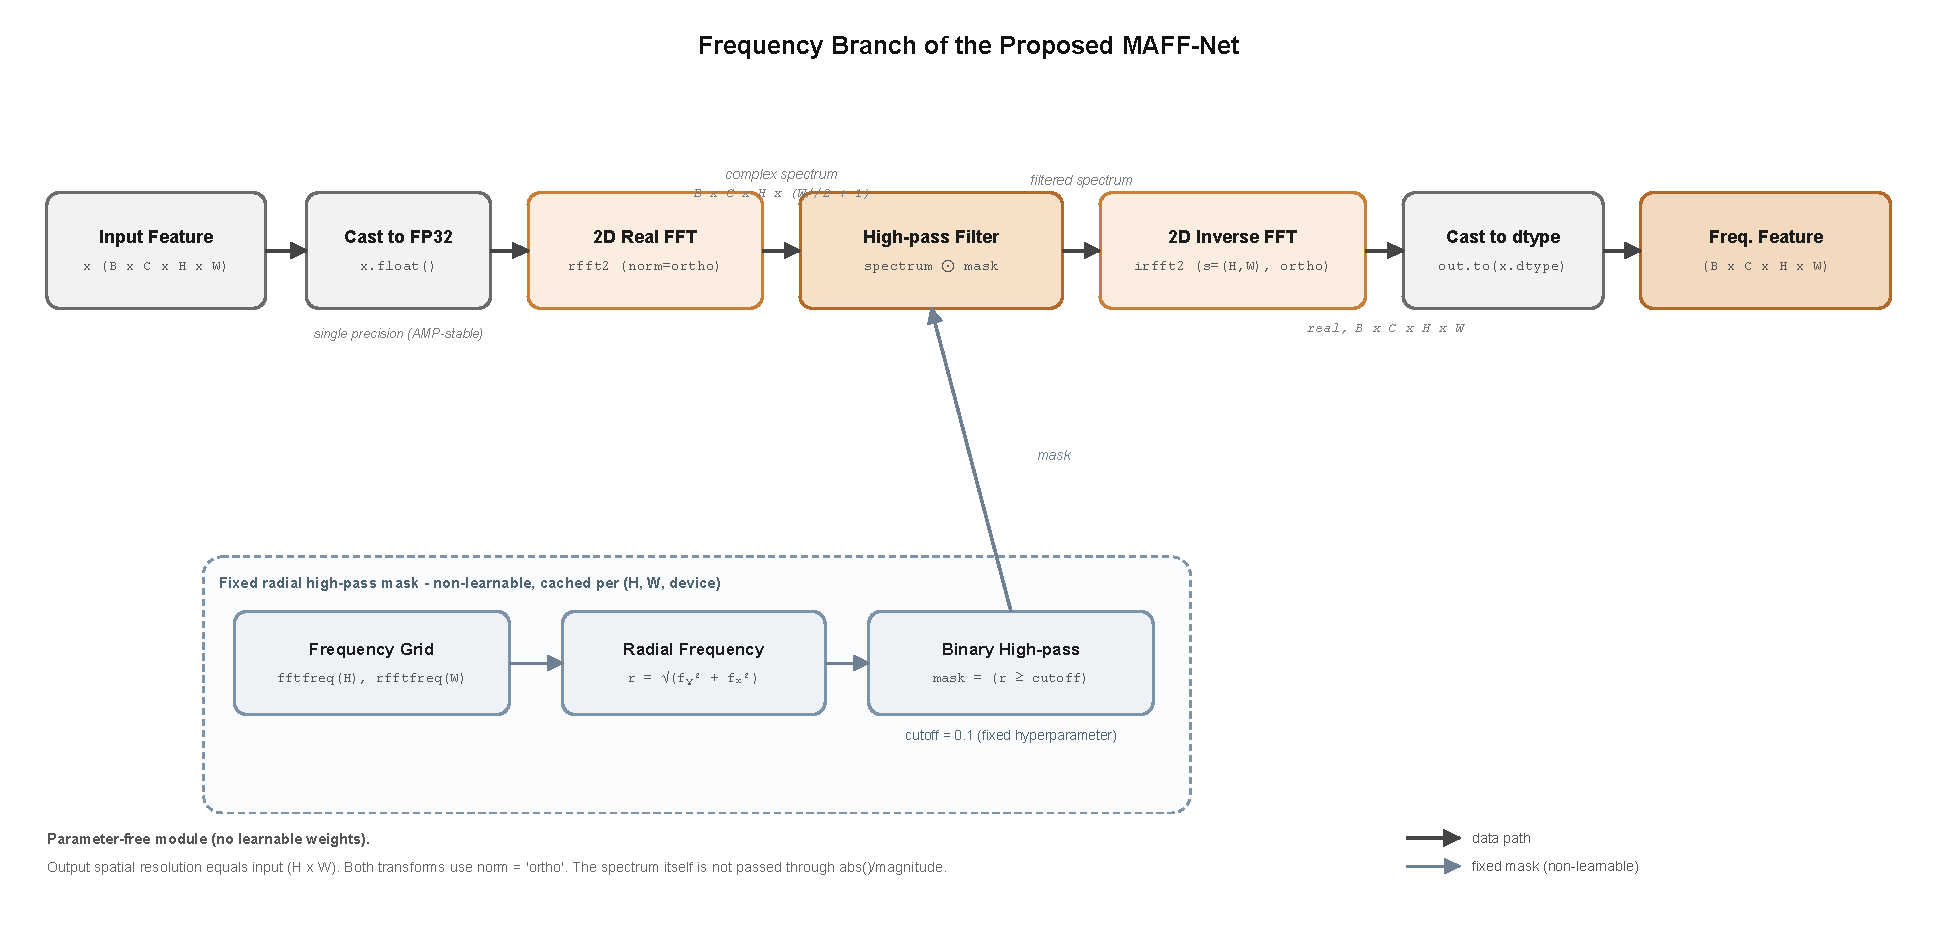
\includegraphics[width=\columnwidth]{Figure2_FrequencyBranch.pdf}
\caption{Internal processing of the Frequency Branch. An input feature is cast
to single precision, transformed by a two-dimensional real FFT, multiplied by a
fixed binary radial high-pass mask with cutoff 0.1, and returned to the spatial
domain by an inverse real FFT at the original resolution. The module is
parameter-free.}
\label{fig:freqbranch}
\end{figure}

The processing follows a single direct path: an encoder feature is mapped into the frequency domain, where its content is expressed in terms of spatial frequencies; the radial high-pass filter suppresses the low-frequency components below the cutoff, which carry the coarse regional appearance, and preserves the high-frequency components that carry edge and fine-detail information; and the filtered representation is returned to the spatial domain as a real-valued output that accentuates the boundary-related structure of the input. Importantly for the surrounding architecture, the spatial resolution of the output matches that of the input feature --- the module neither downsamples nor upsamples --- so the spectral representation remains spatially registered with the feature from which it was derived, and the operation is applied identically at each scale, differing only in the resolution on which it acts.

Within the dual-stream organisation, the Frequency Branch is the frequency-domain counterpart to the spatial pathway: it receives the same multi-scale encoder features supplied to the spatial pathway and operates on them in parallel, so that boundary-sensitive spectral content and contextual spatial content are extracted concurrently from a common source. Its output is not consumed directly by the decoder; at each scale it is passed to a Feature Alignment Module that prepares the spectral representation for combination with its spatial counterpart. This keeps the spectral route explicit and separate up to the point of fusion, in contrast to a design in which spatial and spectral information are combined within a single undifferentiated pathway; and because the module preserves resolution and is applied per scale, its output is spatially compatible with the spatial-stream representation at the corresponding level, a precondition for the subsequent alignment and fusion stages.

A representation obtained purely from high-frequency spectral content differs in its statistical characteristics from a representation obtained in the spatial domain, and these differences must be reconciled before the two can be combined meaningfully. This reconciliation is the responsibility of the Feature Alignment Module, which is applied to the output of the Frequency Branch and, separately, to the spatial representation, and which is described in the following subsection.

\subsection{Feature Alignment Module}

The dual-stream design of the Proposed MAFF-Net produces two representations at every encoder scale --- one from the spatial pathway and one from the Frequency Branch --- that must ultimately be combined into a single representation. Because the two are obtained through different operations, they do not share a common statistical footing, and combining them directly would risk allowing one stream to dominate the other or introducing inconsistencies that the fusion stage cannot resolve. The Feature Alignment Module therefore reconciles the spatial and frequency representations before fusion, bringing them onto comparable terms so that the subsequent combination operates on quantities of similar scale and distribution.

The mismatch arises from the streams' distinct origins. The spatial representation is taken directly from the frozen encoder and carries the full range of content the backbone produces, including the low-frequency and semantic structure describing the lesion interior, so its per-channel statistics reflect that content. The frequency representation, by contrast, is the output of the Frequency Branch, which suppresses the low-frequency components and retains high-frequency structure; it is consequently approximately zero-mean and occupies a different range of values than its spatial counterpart. These differences in per-channel offset, scale, and distribution mean that the two representations are not immediately compatible, and combining them without adjustment would place quantities of dissimilar magnitude on an equal basis.

The module reconciles a representation through a compact, interpretable sequence. It first applies an instance normalisation, which standardises the per-channel statistics on a per-sample basis and thereby removes per-channel offset and scale differences without any learnable parameters of its own. The normalised representation then passes through a learned one-by-one channel projection followed by a rectified-linear activation, which recombines the channels and applies a nonlinearity while retaining a common channel configuration. The learnable content of the module is thus confined to this channel projection, whose weights are updated during training, while the normalisation is a fixed statistical operation. The effect is to place a representation on a normalised, consistently scaled footing suitable for combination with another processed in the same manner.

Within the architecture, the module is instantiated separately for each stream at each encoder scale --- one alignment for the spatial encoder feature and another for the Frequency Branch output, each with its own parameters --- so that at every scale the two streams are aligned independently toward a common form and arrive at the fusion stage on a harmonised statistical footing and a shared channel configuration. Acting only on the encoder features and the Frequency Branch output, it operates entirely downstream of the frozen backbone and leaves it unchanged: the encoder parameters remain fixed, and only the alignment projections are learned. The module thus prepares, rather than combines, the two representations: it establishes the conditions under which a meaningful combination can take place, but leaves the combination itself to a subsequent stage.

With the two representations aligned to a comparable footing at each scale, the network can combine them. That combination is not fixed in advance; the relative contribution of the two aligned streams is determined adaptively by a learned gating mechanism, the Gated Fusion Module, described in the following subsection.

\subsection{Gated Fusion Module}

Once the spatial and frequency representations have been aligned to a comparable footing at each encoder scale, they must be combined into a single representation for decoding. The relative usefulness of the two streams, however, is not uniform: the value of contextual spatial content versus boundary-oriented spectral content varies across images and, within a single image, across spatial locations, since the lesion interior and the region surrounding its boundary place different demands on the two kinds of information. A fixed combination --- concatenation followed by a fixed transformation, or an unweighted summation --- applies the same rule at every position and for every input, so it cannot adjust the balance to local image characteristics and may under-use whichever stream is locally more informative. This motivates the Gated Fusion Module, whose role is to combine the two aligned representations in a manner that adjusts to their content: the weighting between the streams is not prescribed in advance but determined from the features being combined, so that the balance responds to the local content of the representation.

The Gated Fusion Module realises such a combination through a compact gating operation. At each scale, the aligned spatial and frequency representations are concatenated and passed through a single convolutional operation followed by a sigmoid, which produces a gate whose values lie between zero and one and which varies across both channels and spatial positions. The fused representation is then formed as a convex combination of the two aligned representations, in which the gate weights the spatial representation and its complement weights the frequency representation. Because the gate is bounded and its complement is applied to the other stream, the fused output is a proper interpolation between the two aligned representations rather than an unconstrained mixture, and its values remain within the range spanned by its inputs. The gate is computed from the concatenated representations themselves, so the weighting is data-dependent and adjusts to the features presented at each location; the module does not employ an attention mechanism, and its adaptivity is confined to this learned gating. The Gated Fusion Module is illustrated in Fig.~\ref{fig:fafusion}.

\begin{figure}[!t]
\centering
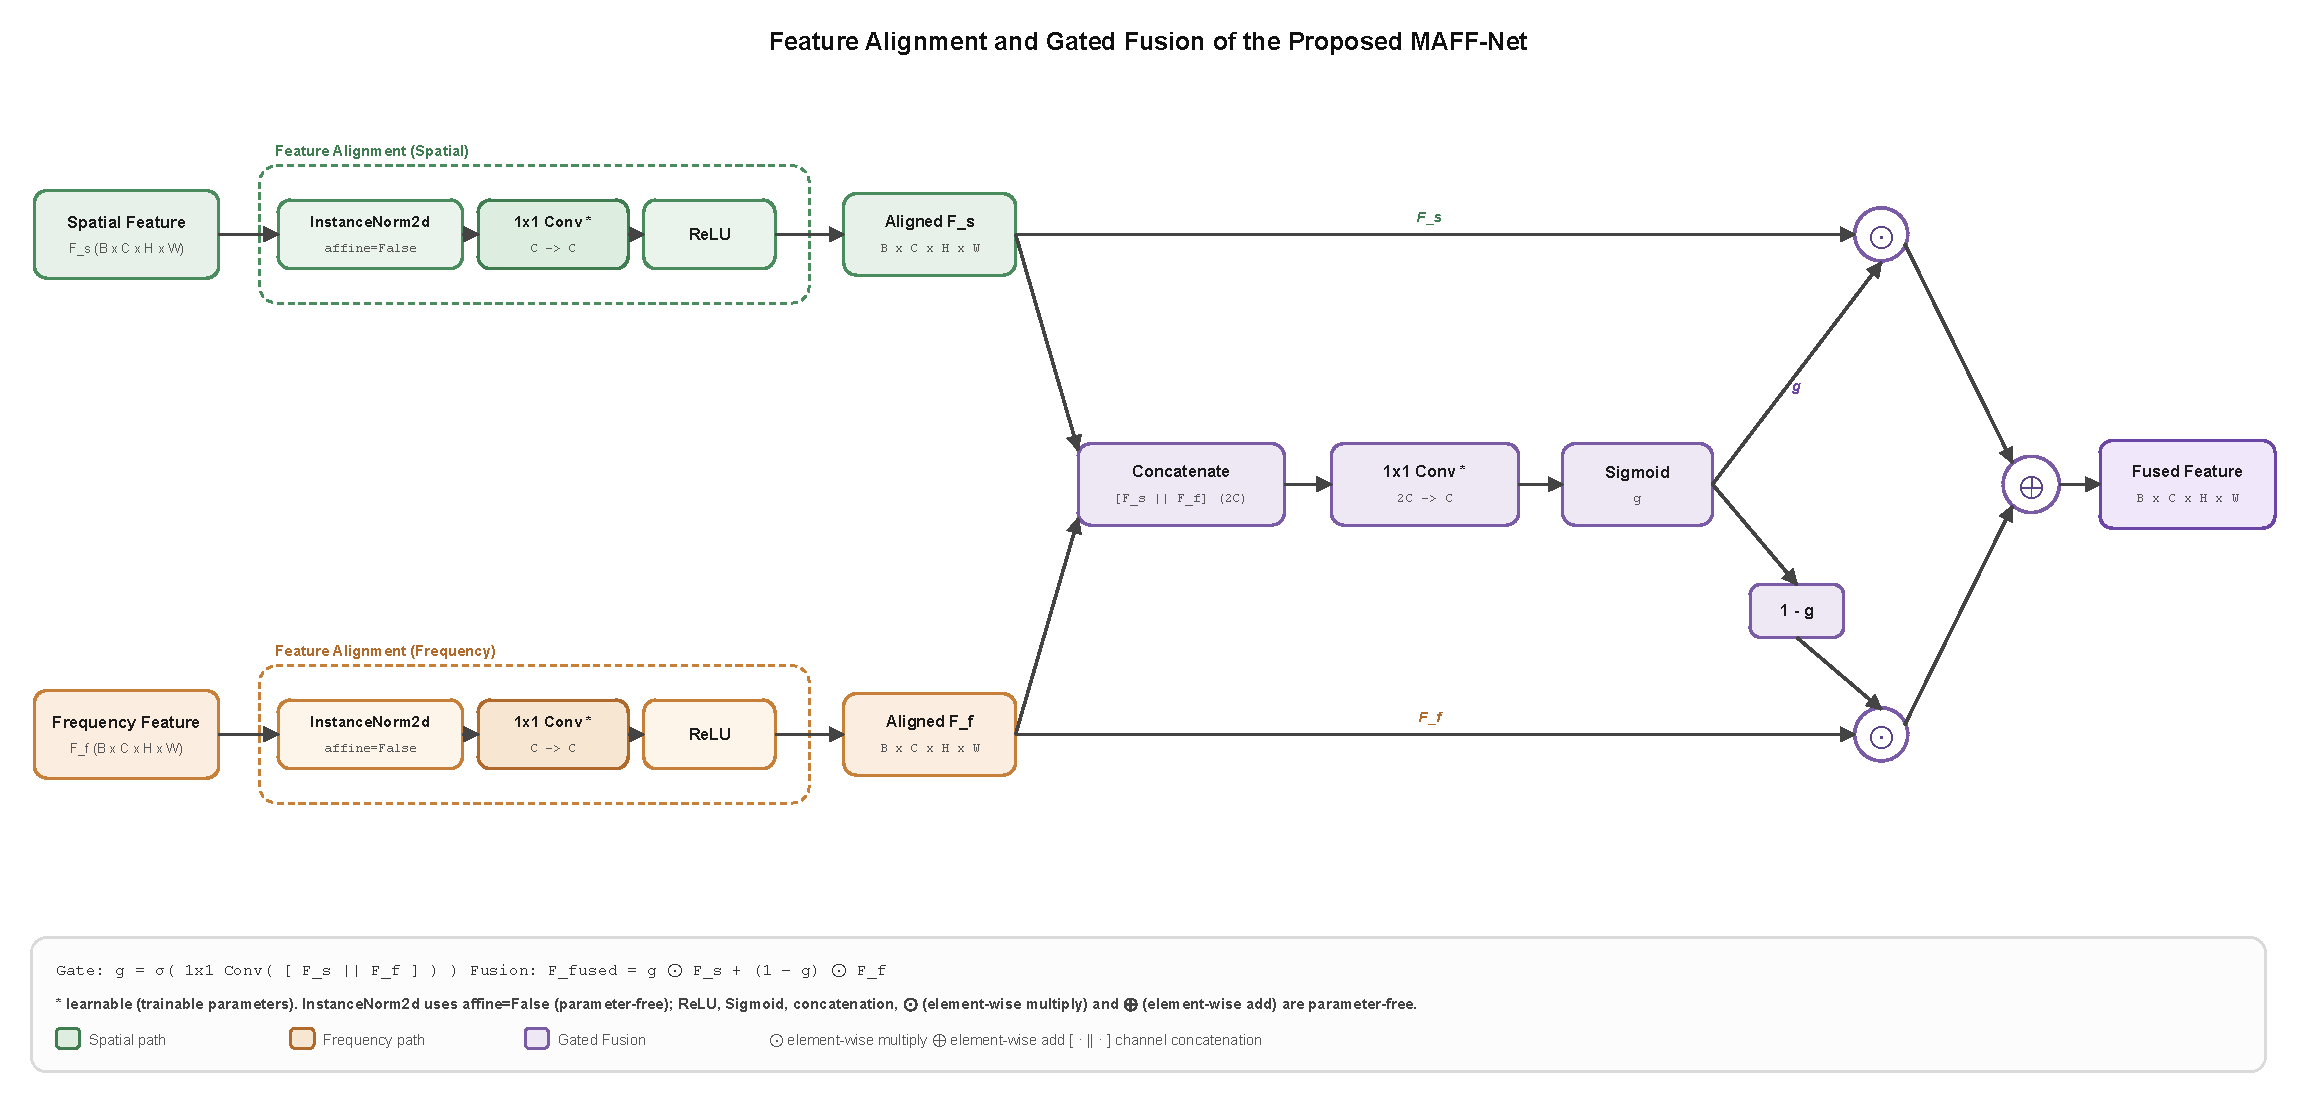
\includegraphics[width=\columnwidth]{Figure3_FeatureAlignment_GatedFusion.pdf}
\caption{Feature Alignment and Gated Fusion. The spatial and frequency features
are aligned independently by instance normalisation, a $1\times1$ convolution,
and a ReLU; the aligned features are then concatenated and passed through a
$1\times1$ convolution and a sigmoid to form a gate $g$, and the fused feature
is the convex combination $g\cdot F_s + (1-g)\cdot F_f$.}
\label{fig:fafusion}
\end{figure}

Within the dual-stream organisation of the Proposed MAFF-Net, the module is instantiated at each encoder scale and receives, at each scale, the two aligned representations produced by the Feature Alignment Module. It is therefore the stage at which the two parallel streams are brought back together: for every scale it consumes an aligned spatial representation and an aligned frequency representation and returns a single fused representation. These fused representations constitute the multi-scale features that the remainder of the network operates on; the deepest fused representation enters the decoder directly as its bottleneck input, while the three shallower fused representations are carried to the decoder through projected skip connections, so that the fused output of each scale contributes to the reconstruction of the segmentation map at the corresponding resolution. In this way the Gated Fusion Module occupies the position between alignment and decoding, converting the two aligned streams into the unified multi-scale representation on which the decoder depends.

With the two aligned streams combined into fused multi-scale representations, the network is ready to reconstruct the segmentation map from these representations. The decoding of the fused features, together with the auxiliary reconstruction branch that accompanies it, both of which are preserved from the Original MAFF-Net, is described in the following subsection.

\subsection{Decoder and Reconstruction Pathway}

Once the Gated Fusion Module has produced a fused representation at each encoder scale, a decoding stage transforms this set of fused multi-scale representations into a full-resolution segmentation prediction. The decoder is the final stage of the Proposed MAFF-Net, progressively resolving the fused features into a dense output at the resolution of the input image. Its decoding pathway is built on the design of the Original MAFF-Net and is not among the scientific contributions of this work; its function is to convert the outputs of the fusion pathway into a segmentation map.

Decoding proceeds hierarchically, from the coarsest fused representation to the finest. Beginning with the fused representation at the deepest scale, the decoder increases spatial resolution stage by stage; at each stage an upsampled higher-level feature is combined with a skip connection carrying information from the corresponding shallower scale, and the combined feature is refined before passing to the next stage. The finest stage refines the representation without a skip connection to complete the recovery of full resolution. Predictions are produced at multiple decoder stages: the highest-resolution one constitutes the segmentation output of the network, while the coarser stages provide additional multi-scale outputs. This coarse-to-fine organisation allows the decoder to recover the overall lesion region at the deeper stages and to sharpen the prediction toward the boundary as resolution increases.

The fused representations produced by the Gated Fusion Module differ from the features a conventional decoder would ordinarily receive, so the decoding pathway is adjusted to accept them: the skip connections entering the decoder are formed by applying a projection to the fused representations before they are combined with the upsampled decoder features, routing the dual-stream outputs into the decoder in a consistent form. This projection and routing are architectural adaptations required to accommodate the fused multi-scale representations; they are engineering adjustments that make the fusion pathway and the decoder compatible, not scientific contributions; the contributions of this work remain the Frequency Branch, the Feature Alignment Module, and the Gated Fusion Module, together with the supervision strategy described next, around which the decoding pathway is adapted.

Alongside the segmentation decoder, an auxiliary reconstruction branch operates on the same fused multi-scale representations and produces an image-sized reconstruction of the input. This provides an auxiliary reconstruction signal that supports training by encouraging the fused representations to retain information about the input. Like the decoder, it follows the design of the Original MAFF-Net, adapted to consume the fused representations rather than reproduced unchanged, and is likewise not claimed as a contribution. The decoder and the reconstruction branch thus draw on the same fused representations for two purposes: the decoder yields the lesion prediction, and the reconstruction branch yields an auxiliary output that regularises the shared representations during training.

The decoder and the reconstruction branch together determine the outputs of the network --- the multi-scale segmentation predictions and the auxiliary reconstruction --- but they do not by themselves specify how those outputs are supervised. The manner in which the multi-scale predictions and the reconstruction are used during training, and in particular the boundary-centric strategy that forms part of the training objective, is the subject of the following subsection on Boundary-centric Dual Supervision.

\subsection{Boundary-centric Dual Supervision}

The primary training signal for the Proposed MAFF-Net is a region-based segmentation objective that measures the agreement between the predicted and reference lesion regions. Such objectives recover the overall extent of a lesion effectively but are comparatively insensitive to errors confined to the boundary, because boundary pixels are few relative to the lesion interior and a small displacement of the contour changes the region-overlap measure only marginally --- a limitation that is particularly consequential in dermoscopy, where margins are frequently diffuse, gradual, or irregular and the clinical value of a segmentation depends heavily on boundary fidelity. To address this without displacing the region objective, the Proposed MAFF-Net augments it with supervision that explicitly targets the lesion contour, referred to as Boundary-centric Dual Supervision. BcDS supplements, rather than replaces, the primary region objective, and comprises two complementary pathways: Boundary-aware Deep Supervision applied to the segmentation outputs, and Edge-weighted Reconstruction applied to the reconstruction branch.

Boundary-aware Deep Supervision acts on the predictions produced by the decoder. The decoder emits predictions at multiple stages under deep supervision, and BDS supervises them by comparing their boundary structure with that of the ground-truth mask, so that discrepancies at the lesion contour are penalised directly. In contrast to the region objective, which compares predicted and reference areas, BDS compares predicted and reference edges, directing learning specifically toward accurate margins rather than overall region agreement. Because it is applied to the same multi-scale predictions that the region objective supervises, BDS adds a contour-oriented signal at each supervised decoder stage while leaving the region objective intact.

Edge-weighted Reconstruction acts on the auxiliary reconstruction branch, whose image-sized reconstruction of the input serves during training as a regularising signal on the shared fused representations. EWR shapes this signal so that the reconstruction discrepancy is emphasised in the regions surrounding the lesion boundary and de-emphasised in the comparatively uniform interior, turning an otherwise region-agnostic reconstruction objective into a boundary-emphasised one. By concentrating the reconstruction pressure along the margins, it encourages the fused representations on which both the decoder and the reconstruction branch depend to retain the boundary-related information that the segmentation prediction requires, reinforcing boundary fidelity indirectly, through the representations, rather than by acting on the prediction itself.

The two pathways impose a shared boundary focus through different outputs of the network, and are complementary rather than duplicative: one supervises what the network predicts at the contour, while the other supervises how well the underlying representations preserve boundary content. Together they constitute the dual character of Boundary-centric Dual Supervision. Both are auxiliary to, and coherent with, the region segmentation objective, sharpening boundary delineation while that objective continues to govern the recovery of the overall lesion region.

Boundary-centric Dual Supervision therefore supervises the multi-scale segmentation predictions and the auxiliary reconstruction with a common emphasis on the lesion boundary, while the region objective remains the primary training signal. The precise formulation of the region objective, the two boundary-focused terms, and the manner in which they are combined into a single training objective is presented in the following subsection.

\subsection{Training Objective / Loss Formulation}

The Proposed MAFF-Net is trained by minimising a single composite objective that combines a primary region-segmentation term with the two auxiliary boundary-focused terms of Boundary-centric Dual Supervision. Let $x$ denote the input dermoscopic image with $C$ channels, $y \in \{0,1\}^{H \times W}$ the binary ground-truth lesion mask, and $p_i$, for $i = 1,\dots,N$ with $N = 4$, the segmentation predictions (as logits) produced at the decoder stages under deep supervision. The logistic sigmoid is written $\sigma(\cdot)$, and sums indexed by $u$ run over spatial locations.

The region term is built from two standard segmentation losses. The soft Dice loss measures the overlap between a predicted probability map and the ground-truth mask,
\begin{equation}
L_{\mathrm{Dice}}(p,y) = 1 - \frac{2\sum_{u}\sigma(p)_u\,y_u + s}{\sum_{u}\sigma(p)_u + \sum_{u}y_u + s}, \tag{1}
\label{eq:1}
\end{equation}
where $s$ is a small smoothing constant that keeps the expression well defined when the mask or prediction is empty. The binary cross-entropy loss, applied to the logits with a positive-class weight $\omega$, measures per-pixel classification agreement,
\begin{equation}
\begin{aligned}
L_{\mathrm{BCE}}(p,y)
&=
-\frac{1}{|\Omega|}
\sum_{u\in\Omega}
\Big[
\omega\,y_u\log\sigma(p)_u
\\
&\qquad
+
(1-y_u)\log\big(1-\sigma(p)_u\big)
\Big].
\end{aligned}
\label{eq:2}
\end{equation}
where $\Omega$ is the set of spatial locations and $\omega$ up-weights lesion (positive) pixels relative to background pixels to counteract class imbalance.

The region objective aggregates these two losses over the deep-supervision predictions: each of the $N$ decoder predictions is supervised with the sum of the Dice and cross-entropy losses, and the results are averaged uniformly,
\begin{equation}
L_{\mathrm{seg}} = \frac{1}{N}\sum_{i=1}^{N}\Big[L_{\mathrm{Dice}}(p_i,y) + L_{\mathrm{BCE}}(p_i,y)\Big]. \tag{3}
\label{eq:3}
\end{equation}
In this uniform average every prediction contributes equally, so the region objective supervises the coarse and fine decoder stages with the same weight.

Boundary-aware Deep Supervision compares the boundary structure of the predictions with that of the ground truth, using an edge operator $S(\cdot)$ that applies the horizontal and vertical Sobel filters $G_x$ and $G_y$, forms the gradient magnitude, and bounds it to the unit interval,
\begin{equation}
S(m) = \mathrm{clamp}\!\Big(\sqrt{(G_x * m)^2 + (G_y * m)^2 + \varepsilon},\,0,\,1\Big), \tag{4a}
\label{eq:4a}
\end{equation}
where $*$ denotes convolution and $\varepsilon$ is a small constant that keeps the gradient of the square root finite in flat regions. The Boundary-aware Deep Supervision loss is then the weighted average, over the deep-supervision predictions, of the discrepancy between the predicted and ground-truth edge maps,
\begin{equation}
L_{\mathrm{BDS}} = \frac{1}{\sum_{i}w_i}\sum_{i=1}^{N} w_i \,\big\lVert\, S\big(\tilde{\sigma}(p_i)\big) - S(y)\,\big\rVert_1, \tag{4b}
\label{eq:4b}
\end{equation}
where $\tilde{\sigma}(p_i)$ is a smoothed sigmoid prediction and $w_i$ are per-prediction weights. Unlike the uniform aggregation of Eq.~\eqref{eq:3}, Eq.~\eqref{eq:4b} weights the predictions, so the finest dominate the boundary term while the coarsest contributes only marginally.

The boundary term is introduced gradually rather than from the first iteration. Its weight follows a linear warm-up schedule,
\begin{equation}
\lambda_{B}(t) = \lambda_{\mathrm{bds}}\cdot\min\!\Big(1,\ \frac{t}{T_{\mathrm{warm}}}\Big), \tag{5}
\label{eq:5}
\end{equation}
where $t$ is the current epoch index, $T_{\mathrm{warm}}$ is the warm-up length, and $\lambda_{\mathrm{bds}}$ is the maximum boundary weight. According to Eq.~\eqref{eq:5}, the weight rises from zero to $\lambda_{\mathrm{bds}}$ over the first $T_{\mathrm{warm}}$ epochs and is constant thereafter, so the region objective governs early training and the boundary term is phased in once the predictions have stabilised.

Edge-weighted Reconstruction supervises the auxiliary reconstruction branch with a boundary-emphasised reconstruction error. A spatial weight map is derived from the ground-truth boundary, $M = 1 + \alpha\,B(y)$, where $B(y)$ is a boundary band obtained from $S(y)$ and $\alpha \ge 0$ controls the emphasis placed on boundary regions. Writing $r$ for the reconstruction mapped to the range of the input image, the loss is a normalised weighted mean-squared error,
\begin{equation}
L_{\mathrm{EWR}} = \frac{\sum_{u} M_u\,(r_u - x_u)^2}{C\sum_{u} M_u}. \tag{6}
\label{eq:6}
\end{equation}
Because $M$ exceeds unity along the lesion boundary and equals unity elsewhere, Eq.~\eqref{eq:6} concentrates the reconstruction pressure on the boundary while normalising by the total weight and the number of channels $C$.

The complete training objective is the weighted sum of the region term and the two boundary terms,
\begin{equation}
L = L_{\mathrm{seg}} + \lambda_{B}(t)\,L_{\mathrm{BDS}} + \lambda_{\mathrm{ewr}}\,L_{\mathrm{EWR}}, \tag{7}
\label{eq:7}
\end{equation}
where $\lambda_{\mathrm{ewr}}$ is the reconstruction weight. In the implemented configuration, the region objective carries unit weight and is the dominant term, with $\lambda_{\mathrm{bds}} = 0.05$ and $\lambda_{\mathrm{ewr}} = 0.05$; the remaining constants are $\omega = 2$, $\alpha = 3$, $T_{\mathrm{warm}} = 5$, and per-prediction weights $w = (1, 1, 1, 0.01)$, with $s$ and $\varepsilon$ set to small fixed values.

The objective in Eq.~\eqref{eq:7} is minimised over the trainable parameters --- the fusion-pathway modules, the decoder, the segmentation heads, and the auxiliary reconstruction branch --- while the encoder remains frozen. Optimisation uses the AdamW optimiser with decoupled weight decay, a learning rate decayed linearly to zero over training, and gradient-norm clipping; training uses mixed-precision autocasting, and the model evaluated is the one with the best validation Dice score. Having specified the training objective, the following section describes the datasets, implementation, and evaluation protocol.

\section{Experimental Setup}
\label{sec:exp}

\subsection{Datasets}

The proposed framework is evaluated on three publicly available dermoscopic skin-lesion segmentation benchmarks released through the International Skin Imaging Collaboration (ISIC): ISIC 2016 \cite{ref20}, ISIC 2017 \cite{ref21}, and ISIC 2018 \cite{ref22}. Each provides dermoscopic images of pigmented lesions with expert-annotated binary masks delineating the lesion from the surrounding skin. The three datasets differ in scale and in the diversity of lesion appearance, and together they span the imaging conditions --- low contrast, diffuse or irregular boundaries, and occlusion by hair --- that motivate the boundary-oriented design of Section III. Evaluating across all three assesses the network under progressively larger and more heterogeneous data rather than on a single collection.

Each dataset is partitioned into disjoint training, validation, and test subsets, and these partitions are held fixed throughout all experiments so that no image contributes to more than one subset. For ISIC 2016 the partition comprises 895 training, 192 validation, and 192 test images; for ISIC 2017, 1600 training, 200 validation, and 200 test images; and for ISIC 2018, 1825 training, 377 validation, and 392 test images. The validation subset is used exclusively for model selection, and the test subset is reserved for final evaluation, never consulted during training or checkpoint selection, so that all reported comparisons are made on data unseen during optimisation.

All images and masks undergo identical preprocessing before training and evaluation. Each image is read as three-channel RGB and each mask as single-channel grayscale, and both are resized to 384$\times$384 pixels --- bilinear interpolation for the images and nearest-neighbour for the masks, which preserves the binary character of the annotations --- after which each mask is binarised at a threshold of one half. During training, and only on the training subset, standard geometric and photometric augmentation is applied: random horizontal and vertical flips, random rotation within thirty degrees, an occasional random affine transformation combining limited rotation, translation, scaling, and shear, and a mild jitter of brightness, contrast, saturation, and hue. The validation and test images are processed without augmentation. Input intensities are standardised to the statistics expected by the frozen encoder within the network, as described in Section III-C, rather than as a dataset-level operation, so that every model receives inputs on a common footing.

\subsection{Implementation Details}

All networks operate on inputs of 384$\times$384 pixels and are trained under a single, consistent configuration, so that differences in behaviour can be attributed to the architectures rather than the training regime. Optimisation uses the AdamW optimiser with decoupled weight decay, an initial learning rate of $1\times10^{-3}$, and a weight decay of $1\times10^{-2}$; the learning rate is annealed linearly to zero over the course of training, and a mini-batch size of two images is used throughout. Training is performed under mixed-precision automatic casting in the bfloat16 format, whose full-range exponent removes the need for gradient loss scaling, and gradients are clipped to a maximum norm of unity at each step. Each model is trained for up to forty epochs; the convolutional baselines are additionally governed by early stopping on the validation Dice score, with a patience of ten epochs, whereas the MAFF-Net family completes the full schedule.

The training objective differs between the two groups of models in accordance with their design. The MAFF-Net family --- the Proposed MAFF-Net together with the Restored MAFF-Net and the Paper-faithful Reconstruction used as reference points --- is trained with the composite Boundary-centric Dual Supervision objective defined in Section III-I. The convolutional baselines are trained with a standard region objective combining the soft Dice loss with a class-weighted binary cross-entropy, the positive class up-weighted to counteract the imbalance between lesion and background pixels. In every case the pretrained SAM2 (Hiera-Large) image encoder \cite{ref10} is retained as a frozen feature extractor, consistent with the role of the backbone established in Section III-C.

All experiments are conducted on a single NVIDIA RTX 2000 Ada Generation graphics processing unit. The software environment comprises Python 3.10, PyTorch 2.7.1 built against CUDA 11.8, on the Windows operating system. The boundary-based metrics introduced below are computed with the MedPy library (version 0.5.2, which relies on SimpleITK) \cite{ref23} together with a direct implementation of the Boundary IoU measure; these are used solely for evaluation and form no part of the training pipeline.

\subsection{Evaluation Metrics}

Segmentation quality is assessed with two complementary families of metrics: the first measures the region overlap between the predicted and reference lesion regions, the second the fidelity of the predicted lesion boundary. Reporting both is essential here because, as argued in Section III-H, region-overlap measures are comparatively insensitive to errors confined to the boundary --- the very behaviour the method is designed to improve. For all metrics, predictions are obtained by applying the logistic sigmoid to the network output and thresholding at one half, using the primary deep-supervision head, and each metric is aggregated over the test set as the mean across evaluation batches, weighted by the number of images per batch. A small constant is added to the denominators to keep every expression well defined when a region is empty.

The region-based metrics are derived from the per-pixel counts of true positives $\mathrm{TP}$, false positives $\mathrm{FP}$, true negatives $\mathrm{TN}$, and false negatives $\mathrm{FN}$ between the thresholded prediction and the binary reference. The pixel accuracy is the overall proportion of correctly classified pixels,
\begin{equation}
\mathrm{Accuracy} = \frac{\mathrm{TP}+\mathrm{TN}}{\mathrm{TP}+\mathrm{FP}+\mathrm{TN}+\mathrm{FN}}, \tag{8}
\label{eq:8}
\end{equation}
the Dice similarity coefficient measures the overlap between the predicted and reference lesion regions,
\begin{equation}
\mathrm{Dice} = \frac{2\,\mathrm{TP}}{2\,\mathrm{TP}+\mathrm{FP}+\mathrm{FN}}, \tag{9}
\label{eq:9}
\end{equation}
and the Intersection-over-Union (IoU), or Jaccard index, provides a related but stricter overlap measure of the lesion region,
\begin{equation}
\mathrm{IoU} = \frac{\mathrm{TP}}{\mathrm{TP}+\mathrm{FP}+\mathrm{FN}}. \tag{10}
\label{eq:10}
\end{equation}
The sensitivity (equivalently, recall) is the proportion of lesion pixels correctly recovered, and the specificity the proportion of background pixels correctly identified,
\begin{equation}
\begin{aligned}
\mathrm{Sensitivity} &= \frac{\mathrm{TP}}{\mathrm{TP}+\mathrm{FN}}, \\
\mathrm{Specificity} &= \frac{\mathrm{TN}}{\mathrm{TN}+\mathrm{FP}}.
\end{aligned} \tag{11}
\label{eq:11}
\end{equation}
The IoU is reported for the lesion (foreground) class; the accuracy, being dominated by the large background region typical of dermoscopic images, is reported for completeness rather than as a primary discriminator.

The boundary-based metrics operate on the contours of the predicted and reference regions. Let $\partial P$ and $\partial G$ denote the boundary pixels of the prediction and the ground truth, and for a point $a$ and a set $S$ let $d(a,S)=\min_{s\in S}\lVert a-s\rVert$ be the Euclidean distance from $a$ to its nearest point in $S$. The average symmetric surface distance (ASSD) is the mean nearest-neighbour distance in both directions between the contours,
\begin{equation}
\mathrm{ASSD} = \frac{\sum_{p\in\partial P} d(p,\partial G) + \sum_{g\in\partial G} d(g,\partial P)}{\lvert\partial P\rvert + \lvert\partial G\rvert}, \tag{12}
\label{eq:12}
\end{equation}
and the 95th-percentile Hausdorff distance (HD95) is the 95th percentile of the same symmetric point-to-contour distances, a robust variant that discounts the most extreme outliers,
\begin{equation}
\mathrm{HD95} = \mathrm{P}_{95}\big(\{\, d(p,\partial G) : p\in\partial P\,\} \cup \{\, d(g,\partial P) : g\in\partial G\,\}\big). \tag{13}
\label{eq:13}
\end{equation}
Both ASSD and HD95 are distance measures for which smaller values indicate closer agreement between the predicted and reference contours; because the images are resized from heterogeneous native resolutions with no physical pixel spacing retained, they are expressed in pixels of the 384$\times$384 evaluation grid rather than in millimetres. The Boundary IoU complements them with an overlap measure restricted to a narrow band around the contour: following the standard formulation \cite{ref12}, a boundary band is obtained for each mask by subtracting its morphological erosion from the mask, the band width being two per cent of the image diagonal, and the IoU is computed between the two bands. Unlike the region IoU, the Boundary IoU is sensitive to contour displacements even when the overall region overlap is large, with larger values indicating better agreement.

\subsection{Experimental Protocol}

The Proposed MAFF-Net is compared against four representative segmentation networks trained and evaluated within the same repository under the protocol described above: the U-Net, the Attention U-Net, the UNet++, and the TransUNet, spanning classical encoder--decoder, attention-gated, nested, and transformer-hybrid designs. They are trained on the identical data partitions, input resolution, and batch size as the proposed model, differing only in the training objective appropriate to each family, as noted in Section IV-B. The Restored MAFF-Net and the Paper-faithful Reconstruction are evaluated under the same protocol and serve as reference points within the MAFF-Net family rather than as external baselines.

A single canonical evaluation protocol is applied uniformly to every model. For each training run the checkpoint achieving the highest validation Dice score is retained and carried forward to evaluation; no test-set information influences its selection. Each retained checkpoint is then evaluated once on the held-out test subset of the corresponding dataset, and the region-based and boundary-based metrics of Section IV-C are computed from the same predictions, using the same thresholding and aggregation. Applying this shared procedure to every model, baseline and proposed alike, ensures that the reported differences reflect the models rather than differences in measurement.

The architectural contributions of the Proposed MAFF-Net are examined through a component ablation on ISIC 2018, the largest and most heterogeneous of the three benchmarks. The ablation follows a leave-one-out design: the complete Proposed MAFF-Net is the reference configuration, and three further configurations each disable exactly one component --- the Frequency Branch, the Feature Alignment Module, and the Gated Fusion Module. The disabled component is replaced by a shape-preserving substitute that leaves the rest of the network and its tensor dimensions unchanged --- the Frequency Branch and the Feature Alignment Module by identity mappings, and the learned gate of the Gated Fusion Module by a fixed, unweighted mean of the two streams --- so that the effect of each component can be isolated. Every ablated configuration is trained with the identical configuration used for the Proposed MAFF-Net and evaluated with the same canonical protocol and metrics, while the reference configuration reuses the existing Proposed MAFF-Net checkpoint without retraining. The frozen encoder, decoder, and reconstruction branch are held fixed across all configurations, so that the study measures only the components introduced in this work.

The following section reports these experiments: first the comparison of the Proposed MAFF-Net with the baselines under the region-based and boundary-based metrics, then the component ablation on ISIC 2018.

\section{Results}
\label{sec:results}

\begin{figure*}[!tp]
\centering
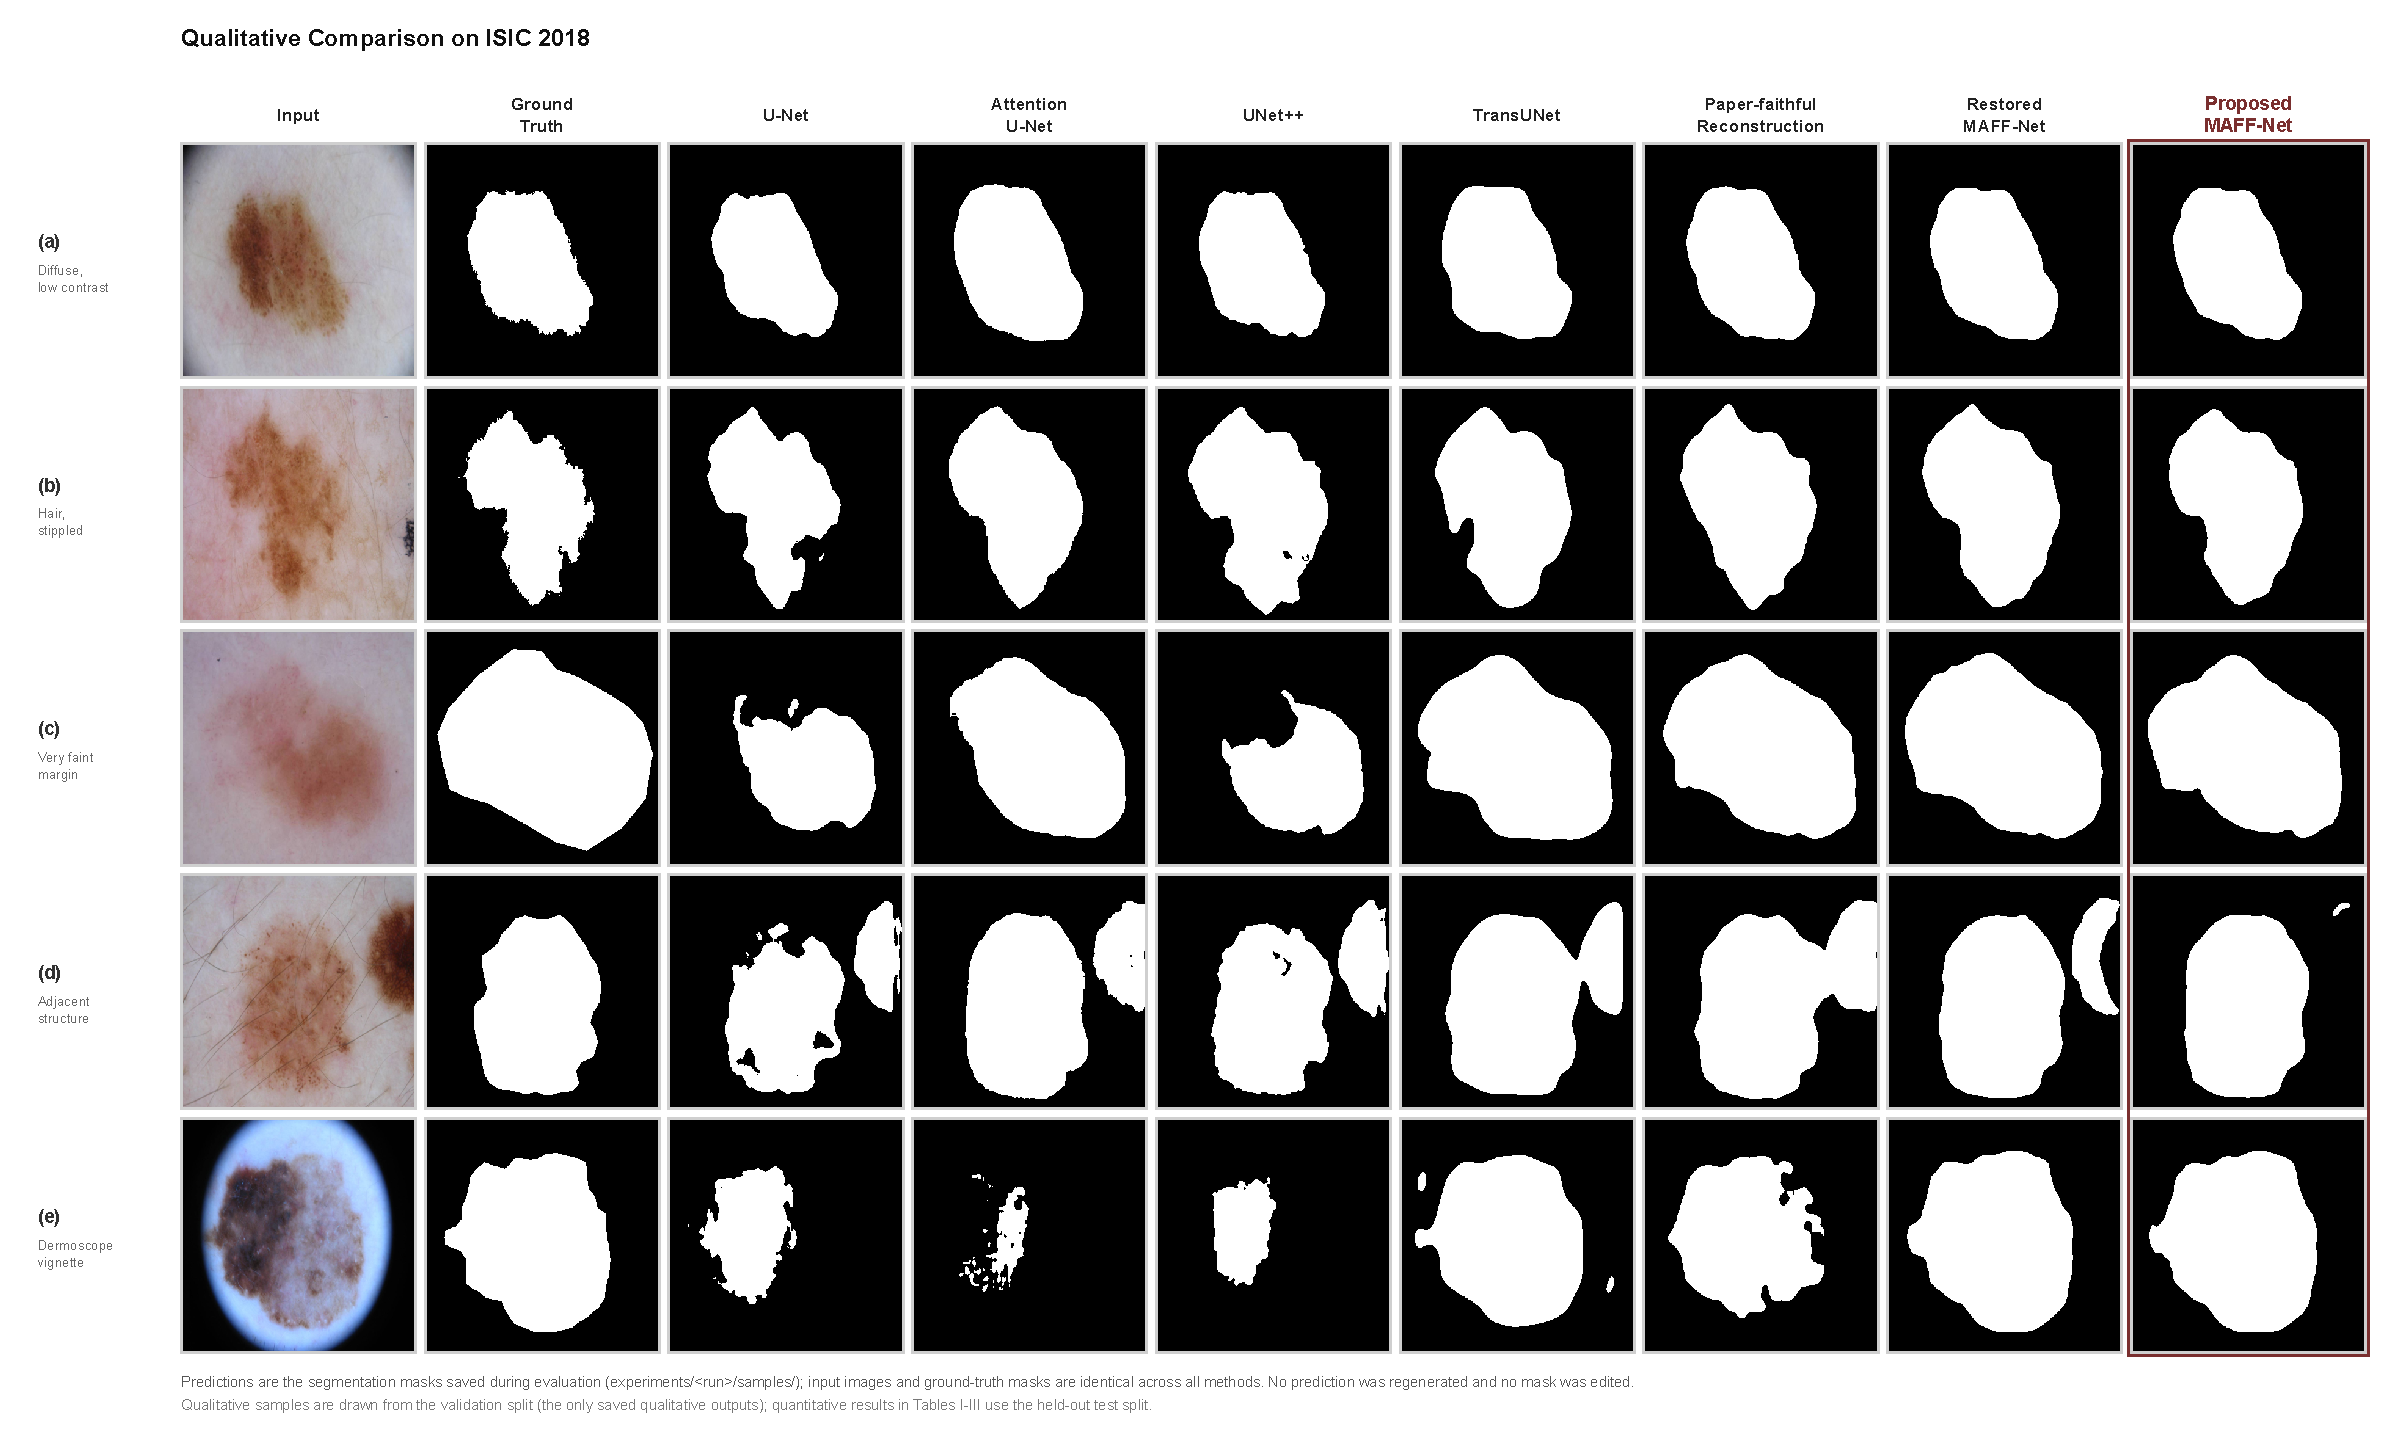
\includegraphics[width=\textwidth]{Figure4_QualitativeComparison.pdf}
\caption{Qualitative comparison on ISIC 2018. Each row is a test case and each
column a method, evaluated on identical input images and ground-truth masks; the
outlined column is the proposed model. Predictions are shown without
modification. The qualitative samples are drawn from the validation split.}
\label{fig:qualitative}
\end{figure*}

\subsection{Benchmark Comparison}

Table~\ref{tab:benchmark} reports the region-based segmentation performance of every evaluated model on the held-out test subsets of ISIC 2016, ISIC 2017, and ISIC 2018 --- the four baseline networks (U-Net, Attention U-Net, UNet++, and TransUNet) and the three members of the MAFF-Net family (the Paper-faithful Reconstruction, the Restored MAFF-Net, and the Proposed MAFF-Net). The Dice coefficient and the IoU are the principal indicators, with accuracy, sensitivity, and specificity reported alongside. Fig.~\ref{fig:region} presents these results graphically.

\begin{figure*}[!t]
\centering
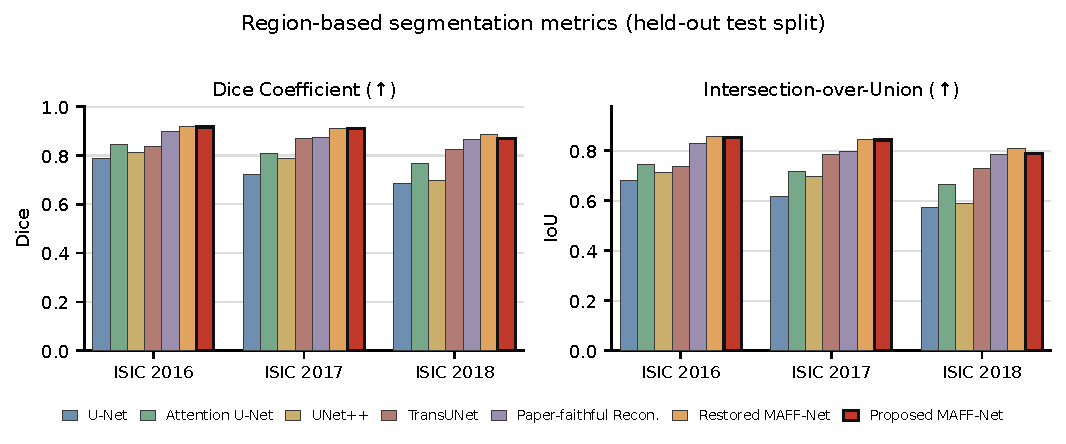
\includegraphics[width=\textwidth]{Figure5_RegionMetrics.pdf}
\caption{Region-based segmentation metrics (Dice and IoU) on the held-out test
splits of ISIC 2016, ISIC 2017, and ISIC 2018 for all evaluated models,
corresponding to Table~\ref{tab:benchmark}.}
\label{fig:region}
\end{figure*}

\begin{table*}[!t]
\centering
\caption{Region-based segmentation performance on the held-out test subsets of
ISIC 2016, ISIC 2017, and ISIC 2018. The highest value in each column, within
each dataset, is shown in bold.}
\label{tab:benchmark}
\setlength{\tabcolsep}{5pt}
\footnotesize
\begin{tabular}{llccccc}
\toprule
Dataset & Method & Dice & IoU & Accuracy & Sensitivity & Specificity \\
\midrule
\multirow{7}{*}{ISIC 2016}
 & U-Net & 0.7874 & 0.6808 & 0.8951 & 0.7649 & 0.9609 \\
 & Attention U-Net & 0.8466 & 0.7443 & 0.9178 & 0.8780 & 0.9495 \\
 & UNet++ & 0.8141 & 0.7140 & 0.9055 & 0.7996 & 0.9647 \\
 & TransUNet & 0.8365 & 0.7349 & 0.9161 & 0.8077 & \textbf{0.9700} \\
 & Paper-faithful Reconstruction & 0.8989 & 0.8264 & 0.9456 & 0.9096 & 0.9591 \\
 & Restored MAFF-Net & \textbf{0.9183} & \textbf{0.8555} & 0.9541 & \textbf{0.9414} & 0.9545 \\
 & Proposed MAFF-Net & 0.9169 & 0.8517 & \textbf{0.9548} & 0.9220 & 0.9689 \\
\midrule
\multirow{7}{*}{ISIC 2017}
 & U-Net & 0.7229 & 0.6152 & 0.9031 & 0.7211 & 0.9562 \\
 & Attention U-Net & 0.8097 & 0.7159 & 0.9331 & 0.8223 & 0.9737 \\
 & UNet++ & 0.7884 & 0.6959 & 0.9291 & 0.7776 & 0.9784 \\
 & TransUNet & 0.8683 & 0.7843 & 0.9561 & 0.8418 & \textbf{0.9870} \\
 & Paper-faithful Reconstruction & 0.8734 & 0.7975 & 0.9588 & 0.9123 & 0.9681 \\
 & Restored MAFF-Net & \textbf{0.9116} & \textbf{0.8447} & \textbf{0.9700} & \textbf{0.9171} & 0.9807 \\
 & Proposed MAFF-Net & 0.9096 & 0.8421 & 0.9682 & 0.9069 & 0.9842 \\
\midrule
\multirow{7}{*}{ISIC 2018}
 & U-Net & 0.6866 & 0.5714 & 0.8732 & 0.7766 & 0.8948 \\
 & Attention U-Net & 0.7662 & 0.6641 & 0.9207 & 0.8352 & 0.9497 \\
 & UNet++ & 0.6978 & 0.5878 & 0.8912 & 0.7692 & 0.9298 \\
 & TransUNet & 0.8259 & 0.7265 & 0.9259 & 0.8929 & 0.9315 \\
 & Paper-faithful Reconstruction & 0.8655 & 0.7855 & 0.9514 & 0.8779 & 0.9730 \\
 & Restored MAFF-Net & \textbf{0.8844} & \textbf{0.8080} & \textbf{0.9584} & \textbf{0.8973} & 0.9730 \\
 & Proposed MAFF-Net & 0.8701 & 0.7900 & 0.9493 & 0.8733 & \textbf{0.9768} \\
\bottomrule
\end{tabular}
\end{table*}

Among the baselines, the U-Net records the lowest Dice coefficient on all three datasets --- 0.7874, 0.7229, and 0.6866 on ISIC 2016, ISIC 2017, and ISIC 2018 --- with IoU values of 0.6808, 0.6152, and 0.5714. The ordering of the remaining baselines is not constant: on ISIC 2016 the Attention U-Net attains the highest baseline Dice coefficient, 0.8466, ahead of the TransUNet at 0.8365 and the UNet++ at 0.8141, whereas on ISIC 2017 and ISIC 2018 the TransUNet leads, at 0.8683 and 0.8259, followed by the Attention U-Net at 0.8097 and 0.7662 and the UNet++ at 0.7884 and 0.6978. The TransUNet is therefore the strongest baseline on two datasets and the Attention U-Net on the third.

All three members of the MAFF-Net family record higher Dice and IoU values than every baseline on every dataset. The narrowest margin occurs on ISIC 2017, where the Paper-faithful Reconstruction attains 0.8734 and 0.7975 against 0.8683 and 0.7843 for the TransUNet; the widest occurs on ISIC 2016, where the same lowest-scoring member attains a Dice coefficient of 0.8989 against 0.8466 for the Attention U-Net, a difference of 0.0523 (0.0396 on ISIC 2018). Relative to the strongest baseline on each dataset, the Proposed MAFF-Net records higher Dice coefficients by 0.0703, 0.0413, and 0.0442 on ISIC 2016, 2017, and 2018.

Within the family the ordering is consistent across all three datasets. The Restored MAFF-Net records the highest Dice coefficient and IoU of all evaluated models --- Dice 0.9183, 0.9116, and 0.8844 and IoU 0.8555, 0.8447, and 0.8080 on ISIC 2016, 2017, and 2018 --- and the Proposed MAFF-Net records the second-highest, with Dice 0.9169, 0.9096, and 0.8701 and IoU 0.8517, 0.8421, and 0.7900. The Dice differences between the Restored and Proposed MAFF-Net are 0.0014, 0.0020, and 0.0143 on the three datasets, and the Paper-faithful Reconstruction records the lowest Dice and IoU within the family throughout.

The remaining measures do not always follow the Dice ordering. The Proposed MAFF-Net attains the highest accuracy of all models on ISIC 2016, 0.9548 against 0.9541 for the Restored MAFF-Net, whereas the Restored MAFF-Net leads on ISIC 2017 and ISIC 2018, at 0.9700 and 0.9584. For specificity, the Proposed MAFF-Net exceeds the Restored MAFF-Net on all three datasets --- 0.9689 against 0.9545, 0.9842 against 0.9807, and 0.9768 against 0.9730 --- the last being the highest specificity on ISIC 2018, though the TransUNet attains the highest specificity of all models on ISIC 2016 and ISIC 2017, at 0.9700 and 0.9870. For sensitivity, the Restored MAFF-Net records the highest value within the family on all three datasets, at 0.9414, 0.9171, and 0.8973; on ISIC 2018 the TransUNet's 0.8929 exceeds both the Proposed MAFF-Net at 0.8733 and the Paper-faithful Reconstruction at 0.8779.

A consistent trend spans the three benchmarks: every model records its lowest Dice and IoU on ISIC 2018, and every model except the TransUNet its highest on ISIC 2016 (the TransUNet peaks on ISIC 2017). The spread between the strongest and weakest models is also widest on ISIC 2018, where Dice coefficients range from 0.6866 to 0.8844, against 0.7874 to 0.9183 on ISIC 2016. Each value corresponds to a single training run per configuration, so the narrower differences between models should be interpreted with corresponding caution. Finally, the Paper-faithful Reconstruction was trained without pretrained SAM2 weights; its values therefore characterise the reconstructed architecture under this study's training conditions and do not reproduce the results reported for the Original MAFF-Net.

\subsection{Boundary Evaluation}

In dermoscopic segmentation the practical value of a prediction depends heavily on the fidelity of the lesion margin, since the margin determines the measured extent of the lesion and is where annotation and prediction most often diverge. The region-overlap measures reported above, however, are dominated by the comparatively large and homogeneous interior: a contour displaced by a few pixels alters the overlap only marginally, so a model may attain a high overlap score while reproducing the margin imprecisely. Measures defined directly on the contour are therefore required. Table~\ref{tab:boundary} reports the three boundary-based measures of Section IV-C --- the 95th-percentile Hausdorff distance, the average symmetric surface distance, and the Boundary IoU --- for every model on the three datasets, and Fig.~\ref{fig:boundary} presents them graphically.

\begin{figure*}[!t]
\centering
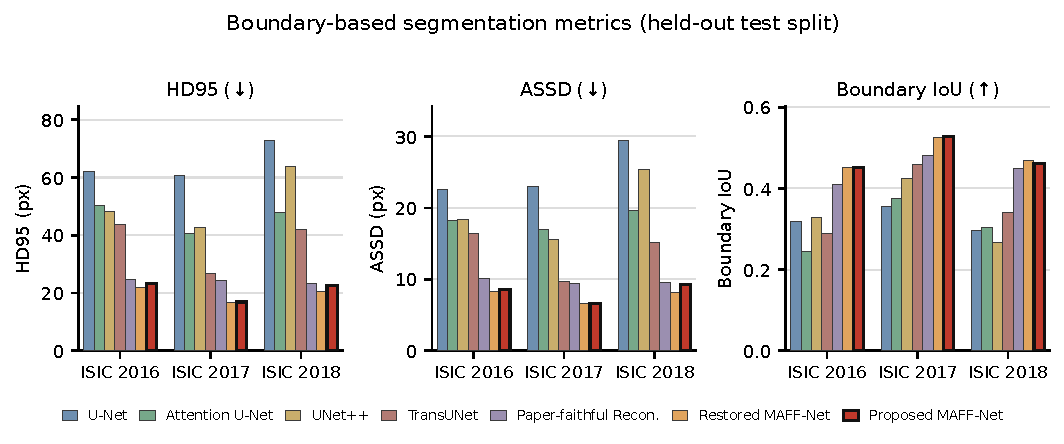
\includegraphics[width=\textwidth]{Figure6_BoundaryMetrics.pdf}
\caption{Boundary-based segmentation metrics (HD95, ASSD, and Boundary IoU) on
the held-out test splits, corresponding to Table~\ref{tab:boundary}. HD95 and
ASSD are in pixels of the $384\times384$ grid and lower is better; higher
Boundary IoU is better.}
\label{fig:boundary}
\end{figure*}

\begin{table*}[!t]
\centering
\caption{Boundary-based segmentation performance on the held-out test subsets of
ISIC 2016, ISIC 2017, and ISIC 2018. HD95 and ASSD are expressed in pixels of
the $384\times384$ evaluation grid, and lower values indicate closer agreement;
higher Boundary IoU values indicate closer agreement. The column
$n_{\mathrm{valid}}$ gives the number of images contributing to the distance
measures. The best value in each column, within each dataset, is shown in bold.}
\label{tab:boundary}
\setlength{\tabcolsep}{6pt}
\footnotesize
\begin{tabular}{llcccc}
\toprule
Dataset & Method & HD95 (px) & ASSD (px) & Boundary IoU & $n_{\mathrm{valid}}/n$ \\
\midrule
\multirow{7}{*}{ISIC 2016}
 & U-Net & 61.976 & 22.527 & 0.3195 & 192 / 192 \\
 & Attention U-Net & 50.465 & 18.221 & 0.2436 & 192 / 192 \\
 & UNet++ & 48.244 & 18.341 & 0.3283 & 190 / 192 \\
 & TransUNet & 43.779 & 16.368 & 0.2898 & 192 / 192 \\
 & Paper-faithful Reconstruction & 24.678 & 10.053 & 0.4101 & 191 / 192 \\
 & Restored MAFF-Net & \textbf{21.979} & \textbf{8.336} & \textbf{0.4518} & 192 / 192 \\
 & Proposed MAFF-Net & 23.329 & 8.510 & 0.4514 & 192 / 192 \\
\midrule
\multirow{7}{*}{ISIC 2017}
 & U-Net & 60.572 & 23.027 & 0.3560 & 194 / 200 \\
 & Attention U-Net & 40.745 & 17.004 & 0.3749 & 198 / 200 \\
 & UNet++ & 42.561 & 15.603 & 0.4244 & 197 / 200 \\
 & TransUNet & 26.750 & 9.710 & 0.4585 & 200 / 200 \\
 & Paper-faithful Reconstruction & 24.210 & 9.409 & 0.4806 & 200 / 200 \\
 & Restored MAFF-Net & \textbf{16.788} & \textbf{6.565} & 0.5255 & 200 / 200 \\
 & Proposed MAFF-Net & 16.869 & 6.645 & \textbf{0.5277} & 200 / 200 \\
\midrule
\multirow{7}{*}{ISIC 2018}
 & U-Net & 72.867 & 29.454 & 0.2958 & 388 / 392 \\
 & Attention U-Net & 47.746 & 19.645 & 0.3035 & 385 / 392 \\
 & UNet++ & 63.710 & 25.348 & 0.2672 & 383 / 392 \\
 & TransUNet & 41.836 & 15.092 & 0.3406 & 392 / 392 \\
 & Paper-faithful Reconstruction & 23.136 & 9.606 & 0.4491 & 390 / 392 \\
 & Restored MAFF-Net & \textbf{20.570} & \textbf{8.199} & \textbf{0.4701} & 392 / 392 \\
 & Proposed MAFF-Net & 22.554 & 9.240 & 0.4611 & 391 / 392 \\
\bottomrule
\end{tabular}
\end{table*}

The distance measures are undefined when a prediction contains no positive pixels; the affected images are excluded from the means and accounted for in the column $n_{\mathrm{valid}}$. Such cases arise for only a minority of images, predominantly among the baselines: the UNet++ produces an empty prediction for nine images of ISIC 2018 and the Attention U-Net for seven, whereas the TransUNet and the Restored MAFF-Net produce none on any dataset and the Proposed MAFF-Net produces one, on ISIC 2018. The Boundary IoU is defined for all images and computed over the complete test subsets.

All three members of the MAFF-Net family record lower HD95, lower ASSD, and higher Boundary IoU than every baseline on each of the three datasets --- the separation holding for all three measures simultaneously and on every dataset, not for an isolated measure or benchmark. Against the strongest baseline for each measure, the Proposed MAFF-Net reduces the HD95 from 43.779 to 23.329 pixels on ISIC 2016, from 26.750 to 16.869 on ISIC 2017, and from 41.836 to 22.554 on ISIC 2018, and the ASSD from 16.368 to 8.510, from 9.710 to 6.645, and from 15.092 to 9.240 pixels on the same datasets. Its Boundary IoU exceeds the highest baseline value by 0.1231, 0.0692, and 0.1205 on ISIC 2016, 2017, and 2018.

Within the family, the Restored MAFF-Net records the lowest HD95 and ASSD on all three datasets --- 21.979 and 8.336 pixels on ISIC 2016, 16.788 and 6.565 on ISIC 2017, and 20.570 and 8.199 on ISIC 2018 --- against 23.329 and 8.510, 16.869 and 6.645, and 22.554 and 9.240 pixels for the Proposed MAFF-Net. For the Boundary IoU the ordering is not uniform: the Proposed MAFF-Net records the highest value of all models on ISIC 2017, 0.5277 against 0.5255, while the Restored MAFF-Net is higher on ISIC 2016, 0.4518 against 0.4514, and ISIC 2018, 0.4701 against 0.4611. The Paper-faithful Reconstruction records the highest distances and lowest Boundary IoU within the family on all three datasets.

The orderings induced by the boundary measures do not coincide with those from region overlap, indicating that region overlap alone does not fully characterise contour quality. On ISIC 2016 the Attention U-Net records the highest Dice coefficient among the baselines yet the lowest Boundary IoU of all models, 0.2436, below the 0.3195 of the U-Net, which has the lowest Dice on that dataset. A comparable disagreement occurs on ISIC 2018, where the UNet++ records a higher Dice than the U-Net, 0.6978 against 0.6866, but a lower Boundary IoU, 0.2672 against 0.2958. Two models may therefore attain similar region overlap while differing appreciably in contour agreement, so the boundary measures provide information the region measures do not.

Three qualifications apply to the values in Table~\ref{tab:boundary}. Each corresponds to a single training run and no statistical testing was performed; the differences between closely ranked models, in particular within the MAFF-Net family, should be regarded as observations on these runs rather than established effects. The per-image dispersion is moreover large relative to the differences between neighbouring models: the standard deviation of the HD95 is of the same order as its mean for every model, ranging from 21.6 to 30.3 pixels within the MAFF-Net family and from 33.9 to 64.8 pixels for the baselines. Finally, as noted in Section IV-C, HD95 and ASSD are in pixels of the 384$\times$384 grid rather than physical units, so they are comparable among the models here but not with distances reported in millimetres elsewhere.

\subsection{Architecture Ablation}

The three components introduced in this work --- the Frequency Branch, the Feature Alignment Module, and the Gated Fusion Module --- were examined by the leave-one-out ablation of Section IV-D, in which each is disabled in turn while the rest of the network and the training configuration are held fixed. The study was conducted on ISIC 2018. Table~\ref{tab:ablation} reports both the region-based and boundary-based measures for the complete model and the three ablated configurations, so that the two families may be considered together.

\begin{table*}[!t]
\centering
\caption{Leave-one-out architecture ablation on the ISIC 2018 test subset. HD95
and ASSD are expressed in pixels of the $384\times384$ evaluation grid, and lower
values indicate closer agreement; higher Dice, IoU, accuracy, and Boundary IoU
values indicate closer agreement. The best value in each column is shown in
bold.}
\label{tab:ablation}
\setlength{\tabcolsep}{6pt}
\small
\begin{tabular}{lcccccc}
\toprule
Configuration & Dice & IoU & Accuracy & HD95 (px) & ASSD (px) & Boundary IoU \\
\midrule
Full Proposed MAFF-Net & 0.8701 & 0.7900 & 0.9493 & \textbf{22.554} & \textbf{9.240} & \textbf{0.4611} \\
without Frequency Branch & 0.8708 & 0.7868 & 0.9496 & 23.574 & 9.546 & 0.4416 \\
without Feature Alignment Module & 0.8649 & 0.7811 & 0.9502 & 23.676 & 9.869 & 0.4326 \\
without Gated Fusion Module & \textbf{0.8725} & \textbf{0.7907} & \textbf{0.9520} & 25.546 & 9.488 & 0.4508 \\
\bottomrule
\end{tabular}
\end{table*}

On the boundary-based measures, the complete Proposed MAFF-Net records the best value of the four configurations on all three: the lowest HD95 at 22.554 pixels, the lowest ASSD at 9.240 pixels, and the highest Boundary IoU at 0.4611. Disabling any one component degrades all three simultaneously: removing the Frequency Branch increases the HD95 by 1.020 pixels and the ASSD by 0.306 and reduces the Boundary IoU by 0.0196; removing the Feature Alignment Module increases them by 1.121 and 0.629 pixels and reduces the Boundary IoU by 0.0286; and removing the Gated Fusion Module increases them by 2.992 and 0.248 pixels and reduces the Boundary IoU by 0.0103. No single component accounts for the whole difference, and the ordering depends on the measure: the largest HD95 increase follows removal of the Gated Fusion Module, the largest ASSD increase and Boundary IoU reduction that of the Feature Alignment Module.

The region-based measures do not separate the four configurations in the same way, and do not favour the complete model. The Dice coefficient varies from 0.8649 to 0.8725, a spread of 0.0076, and the complete model, at 0.8701, does not record the highest value: the configuration without the Gated Fusion Module records the highest Dice at 0.8725, IoU at 0.7907, and accuracy at 0.9520, while the complete model records the lowest accuracy of the four, 0.9493. The only configuration whose Dice falls below the complete model's is the one without the Feature Alignment Module, at 0.8649. The present evidence therefore does not support the proposition that these components improve region overlap, and no such claim is made.

Considered together, the two families indicate that the effect of the three components is confined to the fidelity of the predicted contour rather than the extent of the predicted region. This is consistent with Section V-B, that region overlap is comparatively insensitive to contour displacements: a configuration may reproduce the lesion area to within a small Dice difference while agreeing less closely with the reference contour. On this evidence, the architectural contribution of the present work is accordingly an improvement in boundary fidelity, not in region-overlap performance.

Three qualifications delimit these observations. Each configuration was trained once, with a single experimental seed, and no repeated runs or statistical testing were performed; the differences in Table~\ref{tab:ablation} are therefore observations on these particular runs, not established as statistically significant. The magnitudes are moreover small relative to the per-image dispersion noted in Section V-B, which further limits the weight individual differences can bear. Finally, the study was conducted on ISIC 2018 alone, so the consistency of these observations across the other two datasets is not established here.

\subsection{Qualitative Analysis}

The quantitative measures above summarise agreement over entire test subsets and do not indicate how the predicted contours depart from the reference annotations. Fig.~\ref{fig:qualitative} accordingly presents representative segmentation results on ISIC 2018 for the baselines and the members of the MAFF-Net family, using the same images and annotations for every method so that the predictions may be compared directly. The cases shown are illustrative examples spanning the difficulties of dermoscopic imaging, intended to complement rather than substantiate the quantitative findings.

A characteristic common to all methods concerns the fine structure of the contour. The reference annotations exhibit pixel-level serration along the lesion margin, whereas the predictions of every method, baseline and MAFF-Net variant alike, are comparatively smooth at that scale. None of the models reproduces the finest irregularities of the manual delineation, so the differences observed between methods concern the coarser shape of the contour rather than its fine detail. This applies uniformly and should be borne in mind when assessing the visual results.

For lesions of low contrast and diffuse margin, in which the pigmented region fades gradually into the surrounding skin, the methods differ chiefly in how closely the predicted contour follows the reference outline. The baselines recover the overall extent of such lesions, but their contours tend towards rounded, approximately convex forms --- most evidently the TransUNet, which reproduces the lesion as a compact convex region and does not follow the concavities in the reference outline. The Restored and Proposed MAFF-Net follow the asymmetric form of the reference more closely, reproducing indentations along the margin and the lesion's elongation towards one side, though their contours remain smoother than the annotation at the finest scale.

The methods also differ in the internal consistency of the predicted regions. In several cases examined, the convolutional baselines contain small unsegmented cavities within the lesion interior and isolated fragments detached from the principal region, giving the boundary a broken appearance in places. The MAFF-Net family in the same cases forms closed regions without interior cavities, returning the lesion as a single connected component with a continuous margin. The contours produced by the MAFF-Net variants are correspondingly more regular --- exhibiting fewer isolated fragments and discontinuities, rather than more detail.

The cases containing structures adjacent to the target lesion are the most discriminating. In one, the image is traversed by dense hair and contains a second, darker pigmented structure near the border, excluded by the reference annotation. The U-Net, UNet++, and Attention U-Net each segment this adjacent structure as an additional region, and the TransUNet segments it and connects it to the target lesion, returning the two as one continuous region. The Restored and Proposed MAFF-Net confine the segmentation to the target lesion and return its margin as a closed contour; a residual response to the adjacent structure remains in both, larger for the Restored MAFF-Net and reduced to a small isolated fragment for the Proposed MAFF-Net. The dense hair overlying the lesion does not visibly fragment the MAFF-Net contours, whereas several baselines' margins are locally irregular where the hair traverses.

These observations are subject to clear limitations. They rest on a small number of saved examples per model, drawn from the validation split rather than the test subsets on which the quantitative results were computed, and derive from single training runs. They are consequently illustrative of the models' behaviour on the cases shown, not a representative sample, and do not constitute independent evidence of the differences reported in Sections V-A to V-C. The visual comparison is presented for interpretive value only, and the quantitative measures remain the basis for the comparisons drawn in this work.

\section{Discussion}
\label{sec:discussion}

\subsection{Interpretation of the Component-wise Observations}

The ablation of Section V-C establishes that disabling any one of the three components degrades all three boundary measures simultaneously, while the region measures remain within a narrow band and are not maximised by the complete model. These are marginal effects measured within the Proposed model, each ablated configuration differing from it by a single disabled component; they characterise the role of each component within that model, and are not comparisons with the other members of the MAFF-Net family. The experiments establish that this association exists but do not, by themselves, identify its mechanism, since no analysis of the intermediate representations was undertaken. The accounts below are therefore interpretations consistent with the design of Section III and the observed behaviour, advanced as such rather than demonstrated explanations.

The Frequency Branch applies a fixed radial high-pass filter to each encoder feature and returns the retained content to the spatial domain. Intensity transitions at the lesion margin lie in the higher-frequency spectrum, and a plausible reading of the ablation is that an explicit route for this content preserves margin-associated information that a single representation would otherwise carry with the lower-frequency content of the uniform interior. One aspect of this comparison is unusually clean: the module has no trainable parameters, so replacing it with an identity mapping leaves the network's parameter count unchanged. The degradation that follows its removal therefore cannot be attributed to reduced capacity; in so far as this single-run difference reflects a genuine effect rather than run-to-run variation, it is attributable to the spectral operation itself. This does not establish which spectral content is responsible, only that the operation, not the capacity, would account for such a difference.

Removing the Feature Alignment Module produced the largest degradation in the average symmetric surface distance and the Boundary IoU of the three ablations. The two streams reaching the fusion stage differ in provenance: the spatial stream carries the full encoder feature, whereas the frequency stream, its low-frequency components suppressed, is approximately zero-mean and occupies a different range of values. A reasonable interpretation is that combining representations of dissimilar offset and scale lets one dominate, and that normalising both before the gate is computed allows the weighting to reflect the streams' content rather than their relative magnitudes. This carries an important qualification: the module comprises a normalisation, a learned projection, and a nonlinearity, and disabling it removes all three, so the ablated configuration has slightly fewer trainable parameters than the complete model. The observed degradation cannot be separated, on the present evidence, into the contribution of the normalisation and that of the reduced capacity.

Replacing the Gated Fusion Module with a fixed unweighted mean produced the largest increase in the 95th-percentile Hausdorff distance of the three ablations, but the smallest changes in the average symmetric surface distance and the Boundary IoU. A fixed mean applies the same weighting at every position and input, whereas the gate is computed from the streams themselves and may vary across channels and positions; if the relative usefulness of contextual and margin-associated content differs between the interior and the margin, a position-dependent weighting can reflect that where a fixed rule cannot. That its effect is most pronounced on the 95th-percentile distance, governed by the larger contour deviations, and least on the mean surface distance may indicate that its influence is concentrated on the more severe departures from the reference contour --- a conjecture the present experiments do not test. Here too the ablated configuration has marginally fewer trainable parameters.

\subsection{Boundary Fidelity versus Region Overlap}

That the improvements associated with these components appear in the boundary measures and not in the Dice coefficient follows from a geometric property of the measures, not from any peculiarity of the models: region overlap is area-based, so displacing a contour by a few pixels alters the overlapping area --- and the Dice coefficient --- only slightly, whereas the same displacement enters a contour-distance measure directly and in full. A modification acting principally on the placement of the margin may therefore leave region overlap almost unchanged while producing a measurable change in the boundary measures. The observations of Section V-C are consistent with this: the region measures varied within a narrow band across the four configurations, and the complete model recorded the highest value on none of them, whereas the boundary measures separated the configurations consistently.

Two consequences follow. First, the contribution of the three components is properly characterised as an increase in the fidelity of the predicted contour relative to the configurations in which they are disabled, not as an increase in region-overlap performance; the evidence does not support the latter and no such claim is made. This characterisation is internal to the Proposed model, and is not a claim of superior contour fidelity relative to the other members of the MAFF-Net family, among which, as recorded in Section VI-D, the Restored MAFF-Net attains the closer agreement with the reference contours. Second, region-overlap measures alone are insufficient to characterise methods designed to act on the lesion margin, a point for which Section V-B provides independent support in the disagreement between the two families' orderings. This observation is methodological rather than architectural: it follows from the geometric property noted above rather than any feature of the models, and is therefore expected to bear on the evaluation of other methods intended to act on the object boundary. Both consequences should be weighed against the magnitudes involved, which are small relative to the per-image dispersion of the distance measures.

\subsection{Retaining the Frozen Foundation Backbone}

Retaining the pretrained encoder as a fixed feature extractor carries several advantages here. Its representations are learned from a volume and diversity of data the available dermoscopic collections do not approach, which is material given the size of the datasets employed. Because the encoder is not updated, the trainable capacity is concentrated in the downstream modules and forms a small fraction of the total parameter count, reducing the number of parameters that must be estimated from the comparatively limited annotated data.

A further advantage is methodological. Because the same frozen encoder is used by the Proposed MAFF-Net, the Restored MAFF-Net, and every ablated configuration, the features entering the fusion pathway are identical across them, so differences in behaviour can be attributed to the modules under study rather than feature extraction, which permits the ablation of Section V-C to be read as an assessment of the components themselves; an architecture that also adapted the backbone would not support that inference as directly. The same reasoning applies to the Proposed-versus-Restored comparison: because the two share the frozen encoder and differ only in the fusion pathway, the difference between them in Sections V-A and V-B is attributable to the fusion design rather than feature extraction. On these benchmarks the dual-stream fusion does not surpass the multi-scale perception adaptation and frequency-guided feature fusion of the Original MAFF-Net, and the dual-stream reformulation is accordingly to be understood as an alternative fusion design examined and analysed here rather than one demonstrated to improve upon the original.

These advantages should not be overstated. The experiments include no configuration in which the encoder is fine-tuned, so the comparative merits of freezing and fine-tuning are not assessed here; the rationale rests on the considerations above rather than on evidence produced by this study. As noted in Section V-A, the Paper-faithful Reconstruction was trained without pretrained encoder weights, so the comparison between it and the remaining members of the family does not isolate the effect of the pretrained backbone.

\subsection{Limitations}

Several limitations qualify the findings of this work and delimit the conclusions properly drawn from them.

Each configuration was trained once, with a single seed, and none was repeated. The differences between closely ranked models --- in particular those separating the MAFF-Net family and the four ablated configurations --- are small relative to the per-image dispersion of the measures, so it is not possible, on the present evidence, to distinguish them from the variation between repeated runs. No statistical analysis was performed: no confidence intervals were estimated and no hypothesis tests conducted, and no claim of statistical significance is made anywhere in this work. Repeated runs across several seeds, with an appropriate interval estimate, would be required before the smaller differences reported here could be regarded as established.

The supervision strategy of Section III-H was active in every configuration, and its constituent terms were not ablated; the contribution of the boundary-focused supervision terms is therefore unmeasured, and no claim is advanced regarding their individual efficacy. The component ablation of Section V-C addresses the three architectural modules alone, on a single dataset, so the consistency of its findings across the other two benchmarks is not established.

The evaluation is confined to three dermoscopic benchmarks from the same challenge series. All images derive from a single imaging modality and annotation protocol, and the generality of the findings to other modalities, acquisition devices, or patient populations has not been assessed. The comparison is further restricted to models trained and evaluated within this study; no comparison is drawn against the literature, and several methods from Section II were not implemented here.

Finally, the relative standing within the MAFF-Net family should be stated plainly. The Restored MAFF-Net records the higher value on the majority of the measures in Sections V-A and V-B, including the Dice coefficient and the two distance measures on all three datasets. The evidence assembled here therefore does not establish the proposed configuration as the strongest member of the family on these benchmarks; consistent with the contributions stated in Section I, the value of this work lies in the combined region--boundary evaluation and the ranking disagreement it reveals, in the comparison with the standard baselines, and in the controlled analysis of the three components, not in a claim that the proposed configuration is the best available model. The qualitative observations of Section V-D rest on a few validation-split examples and are illustrative only.

\section{Conclusion}
\label{sec:conclusion}

The delineation of the lesion margin is the principal difficulty of dermoscopic segmentation, and the aspect least well served by the region-overlap criteria with which methods are conventionally optimised and assessed. This work has investigated a targeted dual-stream refinement of the MAFF-Net fusion stage, directed at that aspect. The pretrained encoder, the convolutional decoder, and the auxiliary reconstruction branch are retained from the Original MAFF-Net, and the redesign is confined to the fusion pathway. The multi-scale features of the frozen backbone are processed along two parallel streams --- a spatial stream preserving regional and contextual structure, and a parameter-free Frequency Branch providing an explicit spectral route for boundary-sensitive content --- which a Feature Alignment Module reconciles and a Gated Fusion Module combines by a learned, spatially varying weighting. Training uses a region objective supplemented by auxiliary boundary-focused supervision.

Evaluated on three public dermoscopic benchmarks against four segmentation architectures under an identical protocol, all members of the MAFF-Net family exceeded every baseline on both families of measures across all three datasets. A leave-one-out ablation established that disabling any one of the three proposed components degrades all three boundary measures while leaving the region measures substantially unaffected --- the complete model recording the highest value on no region measure --- so their effect is confined to the fidelity of the predicted contour, and the results do not support, and this work does not advance, any claim that they improve region overlap. The proposed configuration was moreover not the strongest member of the MAFF-Net family, the restored variant recording the higher value on the majority of the measures.

Stated conservatively, the contribution of this work is threefold. First, evaluating the models with region-based and boundary-based measures in combination shows that the two families induce different rankings, so that region-overlap criteria alone are insufficient to characterise methods intended to act upon the lesion margin. Second, the proposed dual-stream model attains higher region-based and boundary-based scores than four standard convolutional and transformer baselines on all three benchmarks under an identical single-run protocol. Third, the dual-stream reformulation of the fusion pathway is investigated and the marginal role of its three components isolated through a controlled leave-one-out ablation, whose results confine the effect of these components to boundary fidelity rather than the extent of the predicted region. No comparison was drawn against results in the literature, and no claim of state-of-the-art performance is made.

The principal limitations indicate the directions in which the study should be extended. Every configuration was trained once, with a single experimental seed, and no statistical analysis was undertaken; repetition across several seeds, with appropriate interval estimates, is required before the smaller differences reported here can be regarded as established, and is the most immediate priority. The evaluation is confined to three benchmarks from a single imaging modality and annotation protocol, so assessment on further collections, and on other modalities and acquisition conditions, is needed to establish generality. Finally, the boundary-focused supervision terms were active in every configuration and were not ablated, so their individual contribution remains unmeasured; ablating them, and examining alternative formulations and their interaction with the architectural components, is a natural continuation of this study.


% ---- Bibliography ----------------------------------------------------------
\bibliographystyle{IEEEtran}
\bibliography{references}

\end{document}
